%==============================================================================
% Homogeneous Three-Topology Comparison and Mode Dictionary
% in Einstein-Cartan + Nieh-Yan Theory: Geometric Structure of EC-Weyl Coupling
%==============================================================================
\documentclass[12pt,a4paper]{article}

%------------------------------------------------------------------------------
% Packages
%------------------------------------------------------------------------------

% Fonts / encoding
\usepackage[T1]{fontenc}
\usepackage{lmodern}
\usepackage{textcomp}
\usepackage[final]{microtype}

% Math
\usepackage{amsmath,amssymb,amsfonts,amsthm}
\usepackage{mathtools}
\usepackage{bm}

% Graphics and figures
\usepackage{graphicx}
\usepackage{float}
\usepackage{subcaption}

% Tables
\usepackage{booktabs}
\usepackage{tabularx}
\usepackage{array}
\usepackage{multirow}

% TikZ for diagrams
\usepackage{tikz}
\usetikzlibrary{shapes.geometric, arrows.meta, positioning, calc, fit, backgrounds}

% Layout and formatting
\usepackage[margin=2.5cm]{geometry}
\usepackage{setspace}
\onehalfspacing

% Misc (xcolor before hyperref)
\usepackage{xcolor}
\usepackage{enumitem}

% References and links
\definecolor{linkblue}{RGB}{0,0,180}
\usepackage[colorlinks=true,linkcolor=linkblue,citecolor=linkblue,urlcolor=linkblue]{hyperref}
\usepackage{cleveref}

% Code listings (for appendices)
\usepackage{listings}
\lstset{
  basicstyle=\ttfamily\small,
  breaklines=true,
  frame=single,
  language=Python
}

% Section break
\usepackage{titlesec}
\newcommand{\sectionbreak}{\clearpage}

%------------------------------------------------------------------------------
% Theorem environments
%------------------------------------------------------------------------------
\newtheorem{theorem}{Theorem}
\newtheorem{proposition}{Proposition}
\newtheorem{lemma}{Lemma}
\newtheorem{corollary}{Corollary}
\theoremstyle{definition}
\newtheorem{definition}{Definition}
\theoremstyle{remark}
\newtheorem{remark}{Remark}

%------------------------------------------------------------------------------
% Custom commands
%------------------------------------------------------------------------------
% Math shortcuts
\newcommand{\dd}{\mathrm{d}}
\newcommand{\Veff}{V_{\mathrm{eff}}}
\newcommand{\VEC}{V_{\mathrm{EC}}}
\newcommand{\LC}{\mathrm{LC}}
\newcommand{\EC}{\mathrm{EC}}
\newcommand{\NY}{\mathrm{NY}}
\newcommand{\Vol}{\mathrm{Vol}}
\newcommand{\tr}{\mathrm{tr}}
\newcommand{\Sym}{\mathrm{Sym}}

% Topology notation
\newcommand{\Sthree}{S^3}
\newcommand{\Tthree}{T^3}
\newcommand{\Nilthree}{\mathrm{Nil}^3}
\newcommand{\Sone}{S^1}

% Inner product notation
\newcommand{\innerprod}[2]{\langle #1,\, #2 \rangle}

% Spin labels
\newcommand{\phys}{\mathrm{phys}}

%------------------------------------------------------------------------------
% Title and author
%------------------------------------------------------------------------------
\title{Homogeneous Three--Topology Comparison and Mode Dictionary in Einstein--Cartan + Nieh--Yan Theory: Geometric Structure of EC--Weyl Coupling}

\author{Muacca}

\date{}

%==============================================================================
\begin{document}
%==============================================================================

\maketitle
\begin{center}
Version: v1\\
First release: 2026-04-06\\
\end{center}

%------------------------------------------------------------------------------
% Abstract
%------------------------------------------------------------------------------
\begin{abstract}
We systematically analyse the homogeneous minisuperspace of gravity with
Einstein--Cartan (EC) connection and Weyl-squared coupling $\alpha C^2_\EC$
across three spatial topologies---$\Sthree\times\Sone$, $\Tthree\times\Sone$,
and $\Nilthree\times\Sone$---and determine how the EC--Weyl coupling modifies
the mode dictionary of each topology.  Extending the Levi--Civita framework of
papers~I--III to the EC connection $\omega_\EC = \Gamma_\LC + K$ (with $K$ the
contortion), we classify torsion modes as axial-scalar (AX), vector-trace (VT),
and their product (MX), and establish nine theorems.

\textbf{Theorem~1 (AX/VT dropout):}  In all three topologies,
$C^2_\EC = C^2_\LC$ holds exactly in the AX ($V=0$) and VT ($\eta=0$)
backgrounds; the EC correction appears only in the MX background as
$C^2_\EC = C^2_\LC + 16V^2\eta^2/(3r^2)$.

\textbf{Theorem~2 (Palatini protection, EC):}  $G^{\EC}_{\eta\eta} =
G^{\EC}_{VV} = 0$ holds algebraically; torsion remains non-propagating
and the spin-2 kinetic structure is unchanged from the LC case.

\textbf{Theorem~3 ($\delta$-sector null theorem):}  The auxiliary cubic
coefficient $C_\delta := \partial^3\Veff/\partial\delta_0\partial\delta_1
\partial\delta_2|_{\delta=0}$ vanishes exactly in all three topologies and all
torsion backgrounds, and $\partial_\alpha C_\delta = 0$.

\textbf{Theorem~4 (Palatini universality):}  In $\Sthree\times\Sone$ the AX
and VT spin-2/spin-1 mass spectra are identical: spin-2 mass
$\mu^2 = 128\pi^2 Lr/(3\kappa^2) - 16384\pi^2 L\alpha/(3r)$ (five-fold
degenerate) and spin-1 mass $m^2_\omega = 16\pi^2 L^3/(\kappa^2 r)$
(three-fold degenerate).

\textbf{Theorem~5 (torsion--volume coupling):}  In $\Tthree\times\Sone$,
$\partial^2\Veff/\partial\varepsilon\partial s|_0 = 48\pi^4 L\eta^2r/\kappa^2
\neq 0$; the cross-term is of purely kinematic origin, independent of the Weyl
mass.

\textbf{Theorem~6 ($\Nilthree$ EC false vacuum):}  For $\alpha<0$,
$\Nilthree\times\Sone$ supports a positive false vacuum at
$r_0 = (4\kappa/\!\sqrt{3})\sqrt{|\alpha|}$ on the $\eta=V=0$ section, with
scaling exponent $\gamma=1/2$.

\textbf{Theorem~7 ($\Nilthree$ quintet splitting):}  The spin-2 quintet around
the EC false vacuum splits as $5\to 0+2+1+1$; the zero mode $q_3$ is
geometrically protected by the one-dimensional Lie structure of $\Nilthree$.

\textbf{Theorem~8 (uniaxial mass splitting):}  In the $\Nilthree$ spin-1
sector, $m^2(\omega_2)\neq 0$ (non-commutative direction) while
$m^2(\omega_0)=m^2(\omega_1)=0$ (commutative directions).

\textbf{Theorem~9 ($\varepsilon$-$s$ cross-term classification):}  The origin
of $\partial^2\Veff/\partial\varepsilon\partial s$ differs essentially across
topologies: purely kinematic for $\Tthree$, vanishing for $\Sthree$, and of
pure curvature/Weyl origin for $\Nilthree$.

These results establish a closed comparison framework for the homogeneous bulk
geometric sector in EC+NY theory under the axial+vector-trace torsion ansatz.
\end{abstract}

%------------------------------------------------------------------------------
% Main text
%------------------------------------------------------------------------------
%==============================================================================
% Section 1: Introduction
%==============================================================================
\section{Introduction}
\label{sec:intro}

\subsection{Background}
\label{sec:intro:background}

In paper~I \cite{paper1} we compared $\Sthree\times\Sone$, $\Tthree\times\Sone$,
and $\Nilthree\times\Sone$ within the Einstein--Cartan + Nieh--Yan (EC+NY)
minisuperspace using a unified effective-potential framework, establishing a
topology-dependent phase classification and demonstrating the energetic
dominance of the isotropic $\Sthree\times\Sone$ vacuum.

In paper~II \cite{paper2} we focused on the isotropic $\Sthree\times\Sone$
vacuum and analysed in detail the effect of the Weyl-squared coupling $\alpha
C^2$ \cite{Woodard2015}.  The Pontryagin density $P=\innerprod{R}{\star R}$
\cite{Chandia1997} was shown to vanish identically under the homogeneous ansatz
(``chiral equilibrium''), and conformal protection for $\alpha\le 0$ together
with asymptotic instability for $\alpha>0$ were established, providing the
physical basis for the geometric robustness of the $\Sthree$ vacuum.

In paper~III (LC version) \cite{paper3} we organised the complete set of
homogeneous geometric degrees of freedom of $\Sthree\times\Sone$---spin-0
(radial $r$, torsion scalars $\eta, V$), spin-2 (traceless symmetric quintet
$q_A$), and spin-1 (physical triplet $X_k$ and auxiliary triplet $Y_k$)---into
a unified geometric Landau-EFT.  The Pontryagin protection, the spin-2 phase
diagram, and the physical/auxiliary decomposition of the spin-1 sector were all
integrated into a single framework.  That paper establishes the baseline
homogeneous mode dictionary for $\Sthree\times\Sone$ and the low-order EFT.

The role of paper~III (LC) in the present work is precisely this: it provides
the confirmed baseline mode dictionary and EFT for $\Sthree\times\Sone$, which
the present paper retains while making the EC--Weyl corrections explicit and
extending the comparison to all three topologies.

The objectives of the present paper are to extend this framework from the
Levi--Civita (LC) connection to the Einstein--Cartan (EC) connection, and to
carry out a systematic three-topology comparison.  Specifically, we address:

\begin{enumerate}
  \item What structure does the EC--Weyl coupling $\alpha C^2_\EC$ have with
        respect to the torsion modes (AX/VT/MX)?
  \item Is the Palatini protection (non-propagation of torsion) established in
        LC also preserved in EC?
  \item How does the mode dictionary of the three topologies change in EC?  In
        particular, does $\Nilthree$ exhibit physics unique to EC?
  \item How do the cross-term structures of squash/shear deformations and the
        EC--Weyl coupling reflect the geometric properties of each topology?
\end{enumerate}

Answers to these four questions are given by the combination of exact symbolic
computation with SymPy and analytic proofs, and are summarised as nine theorems.

\subsection{Summary of Main Results}
\label{sec:intro:results}

The main results of this paper are collected in nine theorems (Theorems~1--9).
Here we describe the significance of each and their interrelations.

\textbf{EC--Weyl coupling structure} (\S\ref{sec:ecweyl}): Theorem~1 provides
the fundamental selection rule that the physical effect of the EC extension
appears only in the MX background ($V\eta\neq 0$).  This ``AX/VT dropout''
holds universally across all three topologies and clarifies the geometric
mechanism of EC--Weyl interaction ($V\times\eta$ cross-terms activate the Weyl
component).  Theorem~3 complements this by establishing that no new cubic
channel appears in the formal auxiliary MIXING sector, so the novel cubic
structure of EC is localised in the physical $\eta$-$V$ channel.

\textbf{Protection structure of $\Sthree\times\Sone$} (\S\ref{sec:ecweyl},
\S\ref{sec:s3}): Theorems~2 and~4 show that the mode dictionary of
$\Sthree\times\Sone$ is essentially protected under the transition from LC to
EC.  Palatini protection (Theorem~2) preserves torsion non-propagation, and
Palatini universality (Theorem~4) ensures that the spin-2/spin-1 mode spectrum
is independent of the type of torsion background.

\textbf{Triple triviality of $\Tthree\times\Sone$} (\S\ref{sec:t3}): The
flatness of $\Tthree$ ($C^a_{bc}=0$) makes all spin-2/spin-1 masses zero
(\S\ref{sec:t3:flat}), and algebraic constraints from AX/VT dropout and MX
corrections coexist.  Theorem~5 clarifies that the squash--shear cross-term
seen in $\Tthree$ is a kinematic consequence of the topology-specific
non-volume-preservation, distinct from the Weyl mass.

\textbf{EC-specific physics of $\Nilthree\times\Sone$} (\S\ref{sec:nil3}):
$\Nilthree$ is the only ``non-conformally flat'' manifold among the three
topologies (non-zero background Weyl tensor), and this generates a positive
EC-induced slice minimum on the $\eta=V=0$ section for $\alpha<0$
(Theorem~6).  The low-energy EFT around this slice-minimum branch is organised
through Theorem~7 (quintet splitting) and Theorem~8 (uniaxial mass splitting).

\textbf{Three-topology comparison} (\S\ref{sec:compare}): Theorem~9 classifies
the geometric differences among the three topologies using the squash--shear
cross-term as an indicator.  The $\gamma=1/2$ scaling theorem (\S\ref{sec:compare:gamma})
and the conformal-flatness theorem (\S\ref{sec:compare:conformal}) clarify the
common geometric principle underlying the EC-specific physics of $\Nilthree$.

\subsection{LC$\to$EC Update Summary}
\label{sec:intro:update}

Table~\ref{tab:update} summarises the changes from paper~III (LC) to the present
paper.  ``Preserved'' indicates a structure established in LC that carries over to
EC unchanged; ``New'' indicates a result first made explicit in the EC version.

\begin{table}[H]
\centering
\resizebox{\linewidth}{!}{%
\begin{tabular}{llll}
\toprule
Quantity / Structure & Paper~III (LC) & This paper (EC) & Change \\
\midrule
Palatini protection ($G_{\eta\eta}=G_{VV}=0$) & \checkmark & \checkmark\ (Thm.~2) & \textbf{Preserved} \\
AX/VT dropout & --- & \checkmark\ all 3 topol.\ (Thm.~1) & \textbf{New} \\
Auxiliary $C_\delta$ & --- & $0$ (all 3 topol., Thm.~3) & \textbf{New} (null result) \\
$\Sthree$ spin-2 mass (isotropic pt.) & $48\pi^2$ (conv.\ dep.) & $128\pi^2 Lr/(3\kappa^2)-16384\pi^2 L\alpha/(3r)$ (Thm.~4) & \textbf{Preserved} (conv.\ unified) \\
$\Sthree$ spin-1 mass & Paper~III \S5 & $16\pi^2 L^3/(\kappa^2 r)$ (Thm.~4) & \textbf{Preserved} \\
$\Sthree$ Pontryagin protection (AX, VT) & \checkmark & \checkmark\ ($\alpha$-independent) & \textbf{Preserved} \\
$\Tthree$ all masses & $=0$ (flatness) & $=0$ (Thm.~5 related) & \textbf{Preserved} \\
$\Tthree$ squash--shear cross-term & --- & kinematic origin established (Thm.~5) & \textbf{New} \\
$\Nilthree$ LC vacuum & absent (monotone) & absent (AX/VT: EC-LC diff.\ zero) & \textbf{Preserved} \\
$\Nilthree$ EC slice minimum & --- & $r_0=(4\kappa/\!\sqrt{3})\sqrt{|\alpha|}$ on $\eta=V=0$ (Thm.~6) & \textbf{New} \\
$\Nilthree$ spin-2 splitting & --- & $5\to 0+2+1+1$ (Thm.~7) & \textbf{New} \\
$\Nilthree$ spin-1 mass splitting & --- & $m^2(\omega_2)\neq 0$ (Thm.~8) & \textbf{New} \\
$\varepsilon$-$s$ cross-term classification & --- & full 3-topology classification (Thm.~9) & \textbf{New} \\
\bottomrule
\end{tabular}%
}
\caption{LC$\to$EC update summary.  ``Preserved'' means the LC structure carries
  over to EC; ``New'' means first established in the EC version.}
\label{tab:update}
\end{table}

\subsection{Outline}
\label{sec:intro:outline}

The paper is organised as follows.
\begin{itemize}
  \item Section~\ref{sec:ecweyl} introduces the basic structure of the
        EC--Weyl coupling and establishes Theorems~1--3.
  \item Section~\ref{sec:s3} gives the mode dictionary for $\Sthree\times\Sone$
        (Theorem~4).
  \item Section~\ref{sec:t3} establishes the mode dictionary for
        $\Tthree\times\Sone$ (Theorem~5).
  \item Section~\ref{sec:nil3} develops the mode dictionary for
        $\Nilthree\times\Sone$ (Theorems~6--8).
  \item Section~\ref{sec:compare} performs the three-topology comparison
        (Theorem~9, $\gamma=1/2$ scaling).
  \item Section~\ref{sec:discussion} discusses the physical implications and
        future prospects.
  \item Section~\ref{sec:conclusion} is the conclusion.
  \item Appendix~\ref{app:A} collects notation and conventions; Appendix~\ref{app:B}
        gives the complete EFT coefficient list; Appendix~\ref{app:C} provides the
        detailed derivation of the $\varepsilon$-$s$ cross-term; Appendix~\ref{app:D}
        gives the detailed proof of the auxiliary $\delta$-sector null theorem.
\end{itemize}
   % Introduction
%==============================================================================
% Section 2: EC-Weyl Coupling Structure
%==============================================================================
\section{EC--Weyl Coupling Structure}
\label{sec:ecweyl}

This section introduces the basic structure of the Einstein--Cartan connection
and determines the dependence of the EC--Weyl scalar $C^2_\EC$ on the torsion
modes.  The main results are \textbf{Theorem~1 (AX/VT dropout)},
\textbf{Theorem~2 (Palatini protection, EC)}, and \textbf{Theorem~3
($\delta$-sector null theorem)}.  The first two give the selection rule of the
EC--Weyl coupling and the non-propagation of torsion; the third establishes
that no new homogeneous cubic channel appears in the auxiliary MIXING sector.

\subsection{EC Connection and Contortion}
\label{sec:ecweyl:connection}

In Einstein--Cartan theory the connection $\omega^a{}_b$ is treated as a
variable independent of the metric.  Its difference from the Levi--Civita (LC)
connection $\Gamma^a{}_{bc}$ is parametrised by the contortion $K^a{}_{bc}$:
\begin{equation}
  \omega_\EC^a{}_{bc} = \Gamma^a{}_{bc} + K^a{}_{bc}.
\end{equation}
The contortion is determined from the antisymmetric torsion tensor
$T^a{}_{bc} = 2\omega^a{}_{[bc]}$ by
\begin{equation}
  K_{abc} = \frac{1}{2}\bigl(T_{abc} + T_{bca} - T_{cab}\bigr),
  \qquad
  K_{abc} = -K_{acb}.
\end{equation}

For the homogeneous minisuperspace torsion ansatz we adopt three modes:
\begin{itemize}
  \item \textbf{AX mode}: axial scalar $\eta$ (traceless antisymmetric part of
        torsion), with $V=0$ assumed.
  \item \textbf{VT mode}: vector-trace scalar $V$ (trace part of torsion), with
        $\eta=0$ assumed.
  \item \textbf{MX mode}: coexistence of AX and VT, i.e.\ $V\neq 0$ and
        $\eta\neq 0$.
\end{itemize}
The action is
\begin{equation}
  S = \int\left[\frac{R_\EC}{2\kappa^2}
      + \theta\cdot\mathcal{L}_\NY
      + \alpha\cdot C^2_\EC\right]\sqrt{g}\,\dd^4x,
\end{equation}
where $R_\EC$ is the EC Ricci scalar, $\mathcal{L}_\NY$ is the Nieh--Yan
density \cite{NiehYan1982}, and $C^2_\EC$ is the EC Weyl scalar
\cite{Woodard2015}.  The coupling constants are $\alpha\in\mathbb{R}$ (Weyl)
and $\theta\in\mathbb{R}$ (NY).  The effective potential
$\Veff(r,\eta,V;\alpha,\theta)$ is computed explicitly for each topology (script:
\texttt{proofs/ax\_vt\_dropout\_proof.py}).

\subsection{Theorem~1: AX/VT Dropout}
\label{sec:ecweyl:thm1}

\begin{theorem}[AX/VT dropout]\label{thm:dropout}
  In all of $\Sthree\times\Sone$, $\Tthree\times\Sone$, and
  $\Nilthree\times\Sone$, the following hold as exact symbolic identities
  verified by SymPy\textup{:}
  \begin{enumerate}
    \item \textbf{AX mode} ($V=0$, $\eta\neq 0$):
          $C^2_\EC = C^2_\LC$ (no EC correction).
    \item \textbf{VT mode} ($\eta=0$, $V\neq 0$):
          $C^2_\EC = C^2_\LC$ (no EC correction).
  \end{enumerate}
  In AX and VT backgrounds, the EC--Weyl coupling $\alpha C^2_\EC$ coincides
  exactly with the LC case and no $\alpha$-dependent new contribution appears.
\end{theorem}

\begin{proof}[Proof outline]
  Expanding $C^2_\EC - C^2_\LC$ symbolically for each topology and factoring,
  every EC correction term carries $V\eta$ as a common factor.  Therefore in
  the AX mode ($V=0$) the correction vanishes exactly, and in the VT mode
  ($\eta=0$) it likewise vanishes (SymPy exact zero in all cases).
\end{proof}

\paragraph{Topology-specific forms.}
For $\Sthree\times\Sone$ and $\Tthree\times\Sone$:
\begin{equation}
  C^2_\LC(\Sthree, \Tthree) = 0 \quad (\text{isotropic point, AX/VT background}).
\end{equation}
AX dropout then confirms $C^2_\EC = 0$.

For $\Nilthree\times\Sone$:
\begin{equation}
  C^2_\LC(\Nilthree) = \frac{4}{3R^4} \neq 0
  \quad (\text{non-conformal flatness}),
\end{equation}
and AX dropout gives $C^2_\EC = 4/(3R^4) = C^2_\LC$ (no EC correction).

\paragraph{$\Tthree$ squash+shear null test.}
For $\Tthree$, $C^2_\EC = 0$ holds for all $\varepsilon, s$ because
$C^a_{bc}=0$ identically.  These six cases (3 topologies $\times$ 2 backgrounds)
are all confirmed as exact zero by SymPy (scripts: \texttt{proofs/ax\_vt\_dropout\_proof.py},
\texttt{proofs/t3\_flatness\_null\_test.py}).

\subsection{MX Mode: EC-Specific Weyl Coupling}
\label{sec:ecweyl:mx}

As the converse of Theorem~\ref{thm:dropout}, in the MX background
($V\neq 0,\eta\neq 0$) an EC-specific Weyl coupling appears.

For $\Sthree\times\Sone$ and $\Tthree\times\Sone$:
\begin{equation}
  C^2_\EC = C^2_\LC + \frac{16V^2\eta^2}{3r^2}.
\end{equation}
For $\Nilthree\times\Sone$:
\begin{equation}
  C^2_\EC = C^2_\LC + \frac{16V^2\eta^2}{3R^2}
           = \frac{4}{3R^4} + \frac{16V^2\eta^2}{3R^2}.
\end{equation}
In both cases the additional term is proportional to $(V\eta)^2$, so the
torsion mixing product modifies the effective potential via the EC--Weyl
coupling:
\begin{equation}
  \Delta\Veff^\EC = \alpha\cdot\frac{16V^2\eta^2}{3r^2}\cdot\Vol(M^3\times\Sone).
\end{equation}
This EC-specific term is the source of effective-potential deformation in the
MX background.  Note, however, that the $\Nilthree$ EC slice minimum discussed
in \S\ref{sec:nil3} originates from $C^2_\LC(\Nilthree)\neq 0$ on the
$\eta=V=0$ section, which is independent of this MX term.

\paragraph{Physical interpretation.}
AX/VT dropout means that torsion alone does not generate new contributions to
the Weyl tensor.  The essence of the EC--Weyl interaction lies in the
``mixing product'' $V\times\eta$ of torsion, understood geometrically as the
mechanism by which an asymmetric combination of contortion activates Weyl
components.  This selection rule is universal across all three topologies and
follows from the general algebraic structure of the EC connection.

\subsection{Theorem~2: Palatini Protection (EC Version)}
\label{sec:ecweyl:thm2}

\begin{theorem}[Palatini protection, EC]\label{thm:palatini}
  Under the Einstein--Cartan connection,
  \begin{equation}
    G^{\EC}_{\eta\eta} = G^{\EC}_{VV} = 0
  \end{equation}
  holds exactly, where $G^{\EC}_{AB} =
  \partial^2\mathcal{L}_\EC/\partial(\partial_z\Phi^A)\partial(\partial_z\Phi^B)$
  is the field-space metric (kinetic metric) of the minisuperspace.
\end{theorem}

\begin{proof}[Proof outline (velocity method)]
  The EC Weyl scalar in the MX background,
  $C^2_\EC(\Sthree, \Tthree, \text{MX}) = 16V^2\eta^2/(3r^2)$,
  is an algebraic function of $(r,\eta,V)$ and contains no velocity fields
  $\partial_z\eta$, $\partial_z V$.  Therefore, computing $G_{\eta\eta}$,
  $G_{VV}$ by the velocity method yields only terms that vanish in the
  $\Delta z\to 0$ limit, and no kinetic term for torsion is generated.
  Full symbolic verification for each topology is given in script
  \texttt{proofs/palatini\_protection\_proof.py}.
\end{proof}

\paragraph{Invariance of $r$-stiffness.}

\begin{table}[H]
\centering
\begin{tabular}{lccc}
\toprule
Topology & $G_{rr}$ (LC) & $G_{rr}$ (EC) & Difference \\
\midrule
$\Sthree$ & 59.22 & 59.22 & 0 \\
$\Tthree$ & 4675.6 & 4675.6 & $\approx 0$ \\
$\Nilthree$ & 5195.2 & 5195.2 & $\approx 0$ \\
\bottomrule
\end{tabular}
\caption{Kinetic metric $G_{rr}$ for the radial mode: LC vs.\ EC.  The
  graviton kinetic structure is unchanged under the EC extension.}
\label{tab:Grr}
\end{table}

The kinetic structure of the spin-2 graviton is also invariant under EC.

\subsection{Theorem~3: $\delta$-Sector Null Theorem}
\label{sec:ecweyl:thm3}

In the EC extension, the new nonlinear coupling
\begin{equation}
  \frac{\partial^3 V_\EC}{\partial\alpha\,\partial\eta\,\partial V} \neq 0
\end{equation}
appears in the physical $(\eta,V)$ channel (\S\ref{sec:s3:ec}).  A separate
question is whether an independent cubic channel also arises in the auxiliary
MIXING variable $\delta_k$.  We define
\begin{equation}
  C_\delta(M^3;\text{mode}) :=
  \left.\frac{\partial^3\Veff}{\partial\delta_0\,\partial\delta_1\,\partial\delta_2}
  \right|_{\delta_0=\delta_1=\delta_2=0},
\end{equation}
where $M^3 = \Sthree, \Tthree, \Nilthree$ and mode $=$ AX/VT/MX.

\begin{theorem}[$\delta$-sector null theorem]\label{thm:delta}
  For all three topologies and all torsion backgrounds \textup{(}AX, VT,
  MX\textup{)},
  \begin{equation}
    C_\delta(M^3;\text{mode}) = 0
    \qquad\text{and}\qquad
    \frac{\partial C_\delta}{\partial\alpha} = 0
  \end{equation}
  hold as exact SymPy results.  The EC extension generates no new homogeneous
  cubic channel in the auxiliary $\delta$-sector.
\end{theorem}

\begin{proof}[Proof outline]
  With \texttt{fiber\_mode = MIXING} activated in the unified engine, we
  construct $\Veff$ for each topology and torsion background, then compute the
  third derivative $\partial_{\delta_0}\partial_{\delta_1}\partial_{\delta_2}\Veff|_{\delta=0}$
  by direct symbolic differentiation.  All nine cases give exact zero
  coefficients, from which $\partial_\alpha C_\delta = 0$ follows automatically.
  The key point is not that EC has no new effects, but that the new cubic
  structure activated by EC is localised in the physical $\eta$-$V$ channel
  rather than the auxiliary $\delta$-sector.
\end{proof}

\paragraph{Topology-wise consequences.}
\begin{itemize}
  \item $\Sthree$: The formal MIXING sector is nontrivially available, yet
        $C_\delta(\Sthree)=0$.  Hence the $\alpha$-cubic of \S\ref{sec:s3:ec}
        appears only in the $\eta$-$V$ sector.
  \item $\Tthree$: Flatness trivialises most of the mode dictionary.  Even the
        formal MIXING test gives $C_\delta(\Tthree)=0$.
  \item $\Nilthree$: Despite the non-conformal flatness and the EC false
        vacuum, $C_\delta(\Nilthree)=0$.  The EC-specific physics of $\Nilthree$
        resides in the background Weyl and the $(r,\eta,V)$ sector.
\end{itemize}
Detailed derivations and the exact check of all nine cases are given in
Appendix~\ref{app:D} and script \texttt{proofs/c\_delta\_null\_proof.py}.
   % EC-Weyl Coupling Structure
%==============================================================================
% Section 3: Mode Dictionary: S^3 x S^1 under EC-Weyl
%==============================================================================
\section{Mode Dictionary: $\Sthree\times\Sone$ under EC--Weyl}
\label{sec:s3}

This section determines the effect of the EC--Weyl coupling on the homogeneous
geometric degrees of freedom of $\Sthree\times\Sone$.  Since the non-propagation
of torsion in the spin-0 sector is already established by Theorem~\ref{thm:palatini},
we focus here on the specific consequences for $\Sthree$: Theorem~4 (Palatini
universality) and its reflection in the mode dictionary.

\subsection{Theorem~4: Palatini Universality}
\label{sec:s3:thm4}

\begin{theorem}[Palatini universality]\label{thm:paluniv}
  In $\Sthree\times\Sone$, the spin-2 and spin-1 masses in the AX and VT
  backgrounds are identical (SymPy exact)\textup{:}

  \textbf{Spin-2 mass (five-fold degenerate)\textup{:}}
  \begin{equation}
    \mu^2_{\mathrm{spin2}}(\Sthree)
    = \frac{128\pi^2 Lr}{3\kappa^2} - \frac{16384\pi^2 L\alpha}{3r}.
  \end{equation}

  \textbf{Spin-1 mass (three-fold degenerate)\textup{:}}
  \begin{equation}
    m^2_{\omega_k}(\Sthree) = \frac{16\pi^2 L^3}{\kappa^2 r},
    \qquad k=0,1,2.
  \end{equation}

  Both expressions are independent of $\eta$ and $V$: the mode spectrum does
  not depend on the type of torsion background.
\end{theorem}

The VT$-$AX difference for spin-2 mass is exactly zero (SymPy exact).  The LC
contribution ($\alpha=0$) to the spin-2 mass is $128\pi^2 Lr/(3\kappa^2)$ and
the EC correction is $-16384\pi^2 L\alpha/(3r)$, the latter depending only on
the topology ($\Sthree$ geometry) and not on $\eta$ or $V$.

\begin{remark}
  The numerical evaluation at $r=3$, $L=\kappa=1$, $\alpha=0$ gives
  $\mu^2_{\mathrm{spin2}} = 128\pi^2 \approx 1263.3$ and
  $m^2_{\omega_k} = 16\pi^2/3 \approx 52.6$.  The LC paper~III uses $r=1$-based
  notation, giving $128\pi^2/3\approx 421.2$ for the spin-2 mass.  The
  discrepancy with the value $48\pi^2$ quoted there arises from the choice of
  radius combined with conventions for the spin-2 basis/Hessian.
\end{remark}

\paragraph{Physical interpretation.}
Palatini universality means that the difference between the AX background
($\eta\neq 0$) and the VT background ($V\neq 0$) has no effect on the
spin-2/spin-1 mass spectrum.  The kinematic part coming from the $\Sthree$
geometry ($C^i_{jk}=4\varepsilon_{ijk}/r$) determines the masses, while
torsion deforms only the shape of the potential (a consequence of Palatini
protection, Theorem~\ref{thm:palatini}).
Script: \texttt{paper03ec/s3\_vt\_spin\_masses.py}.

\subsection{Mode Dictionary Table ($\Sthree\times\Sone$)}
\label{sec:s3:table}

Table~\ref{tab:s3} summarises the mode dictionary of $\Sthree\times\Sone$
under EC--Weyl.

\begin{table}[H]
\centering
\resizebox{\linewidth}{!}{%
\begin{tabular}{lccc}
\toprule
Quantity & AX ($V=0,\,\eta\neq 0$) & VT ($\eta=0,\,V\neq 0$) & MX ($V\neq 0,\,\eta\neq 0$) \\
\midrule
$C^2_\EC$ & $=C^2_\LC=0$ & $=C^2_\LC=0$ & $16V^2\eta^2/(3r^2)$ \\
AX/VT dropout & \checkmark & \checkmark & $\times$ \\
spin-0: $r$ & propagating & propagating & propagating \\
spin-0: $\eta,V$ & $\eta$ non-prop., $V=0$ (Thm.~2) & $\eta=0$, $V$ non-prop.\ (Thm.~2) & both non-prop.\ (Thm.~2) \\
spin-2 mass $\mu^2$ & $128\pi^2 Lr/(3\kappa^2)-16384\pi^2 L\alpha/(3r)$ & same as AX (Thm.~4) & --- \\
spin-1 mass $m^2_\omega$ & $16\pi^2 L^3/(\kappa^2 r)$ (3-fold) & same as AX (Thm.~4) & --- \\
\bottomrule
\end{tabular}%
}
\caption{$\Sthree\times\Sone$ mode dictionary under EC--Weyl.}
\label{tab:s3}
\end{table}

Regarding the MX sector of $\Sthree\times\Sone$: the supplementary script \\
\texttt{paper03ec/s3\_mx\_vacuum\_search.py} checked the stationarity conditions
and Hessian within the range $|\eta|\le 3$.  No stable full stationary vacuum
satisfying both $\nabla_{(r,\eta,V)}\Veff=0$ and positive-definite Hessian was
found.  Real stationary points may appear on the $\alpha>0$ side, but all of
them have at least one negative eigenvalue and are saddle points.  The finite-radius
well appearing in a fixed-$V$ slice is a one-dimensional minimum in the $r$
direction and does not constitute a full stationary vacuum.

\subsection{Pontryagin Structure: AX = Pl\"{u}cker, VT = Pfaffian, MX $\neq 0$}
\label{sec:s3:pontryagin}

The Pontryagin protection structure is inherited from paper~III.

\textbf{AX mode (Pl\"ucker protection):} When $V=0$, the Pontryagin density
$P=\innerprod{R}{\star R}$ vanishes identically by a Pl\"ucker relation.
AX torsion contributes no antisymmetric part to the Riemann tensor that could
activate $P$.

\textbf{VT mode (Pfaffian protection):} When $\eta=0$, $P$ vanishes via a
Pfaffian-type identity.  VT torsion modifies only the symmetric part of the
Riemann tensor, leaving the antisymmetric combination that enters $P$ zero.

\textbf{MX mode:} When $V\neq 0,\eta\neq 0$, the Pontryagin density at the
isotropic point is (from paper~III):
\begin{equation}
  P_0 = \frac{2V\eta(V^2r^2 + 9\eta^2 - 36)}{9r^3}.
\end{equation}

\paragraph{Effect of EC.}
The Weyl coupling $\alpha$ enters only the action, not the definition of the
Pontryagin density $P$ itself.  Therefore the AX/VT/MX Pontryagin classification
is unchanged from paper~III, and what changes in the EC extension is the
effective potential $\Veff$ side.

\subsection{EC-Specific Modification under EC--Weyl}
\label{sec:s3:ec}

\textbf{Preservation of AX/VT stability.}
Under EC correction $\alpha<0$, the structure of the AX/VT stable vacua is
unchanged from LC.  By the AX/VT dropout (Theorem~\ref{thm:dropout}),
$C^2_\EC = C^2_\LC$, so the Weyl coupling does not modify the effective
potential.

\textbf{EC-specific cubic coupling ($\alpha$-cubic).}
As a new nonlinear coupling absent in LC, the following appears:
\begin{equation}
  \frac{\partial^3 V_\EC}{\partial\alpha\,\partial\eta\,\partial V}
  = -\frac{128\pi^2 V\eta r}{3} \neq 0
  \qquad (\Sthree).
\end{equation}
This gives the EC-specific cubic coefficient in the homogeneous EFT with respect
to $\alpha$, a cubic channel absent in LC (script:
\texttt{paper03ec/ec\_cubic\_vertex.py}).  This term does not appear in the
second-order mode dictionary of Table~\ref{tab:s3} and enters only at cubic
order in the homogeneous EFT.  The coefficient corresponds to the
$\Sthree\times\Sone$ volume convention $\Vol(\Sthree\times\Sone)=2\pi^2 Lr^3$
of Appendix~\ref{app:A}.  For comparison, the NY-cubic channel
$\partial^3 V/\partial\theta\partial\eta\partial V = 4\pi^2 r^2$ is invariant
under EC (a consequence of Palatini protection).

In the auxiliary formal MIXING sector, on the other hand,
\begin{equation}
  C_\delta(\Sthree) = 0,
  \qquad
  \frac{\partial C_\delta(\Sthree)}{\partial\alpha} = 0
\end{equation}
(Theorem~\ref{thm:delta}, Appendix~\ref{app:D}).  Therefore the new homogeneous
cubic structure activated by EC extension is confined to the physical $\eta$-$V$
channel, and the $\delta$-sector remains null.
   % Mode Dictionary: S3 x S1
%==============================================================================
% Section 4: Mode Dictionary: T^3 x S^1 under EC-Weyl
%==============================================================================
\section{Mode Dictionary: $\Tthree\times\Sone$ under EC--Weyl}
\label{sec:t3}

This section analyses the effect of the EC--Weyl coupling on the homogeneous
geometric degrees of freedom of $\Tthree\times\Sone$.  The flatness of $\Tthree$
($C^a_{bc}=0$) causes a triple triviality, and we establish Theorem~5
(torsion--volume coupling) as the origin of the squash--shear cross-term.

\subsection{$\Tthree$ Flatness Theorem}
\label{sec:t3:flat}

$\Tthree = \mathbb{R}^3/\mathbb{Z}^3$ is a flat torus with
\begin{equation}
  C^a_{bc}(\Tthree) = 0 \quad \forall\,a,b,c.
\end{equation}
This flatness causes the Weyl tensor to vanish, setting all spin-2/spin-1
masses to zero.

\paragraph{Spin-2 mass (squash direction).}
By exact SymPy computation,
\begin{equation}
  \frac{\partial^2 V}{\partial\varepsilon^2}\bigg|_{\varepsilon=0}
  = 0 \quad \forall\,\eta, V, \alpha.
\end{equation}
With $C^a_{bc}=0$, the Weyl tensor vanishes and no geometric mass term for spin-2
arises.  Script: \texttt{paper03ec/t3\_mode\_dictionary.py}.

\paragraph{Spin-2 mass (shear direction).}
Similarly,
\begin{equation}
  \frac{\partial^2 V}{\partial s^2}\bigg|_{s=0}
  = 0 \quad \forall\,\eta, V, \alpha
\end{equation}
(SymPy exact zero; script: \texttt{proofs/t3\_flatness\_null\_test.py}).

\paragraph{Spin-1 mass.}
With $C^a_{bc}=0$, all spin-1 components are massless: $m^2_\omega = 0$.

\subsection{Mode Dictionary Table ($\Tthree\times\Sone$)}
\label{sec:t3:table}

\begin{table}[H]
\centering
\small
\begin{tabular}{lccc}
\toprule
Quantity & AX ($V=0,\,\eta\neq 0$) & VT ($\eta=0,\,V\neq 0$) & MX ($V\neq 0,\,\eta\neq 0$) \\
\midrule
$C^2_\EC$ & $=C^2_\LC=0$ & $=C^2_\LC=0$ & $16V^2\eta^2/(3r^2)$ \\
AX/VT dropout & \checkmark & \checkmark & $\times$ \\
spin-0: $r$ & propagating & propagating & propagating \\
spin-0: $\eta,V$ & $\eta$ non-prop., $V=0$ & $\eta=0$, $V$ non-prop. & both non-prop. \\
spin-2 mass $\mu^2$ & $0$ ($\Tthree$ flatness) & $0$ ($\Tthree$ flatness) & $0$ ($\Tthree$ flatness) \\
spin-1 mass $m^2_\omega$ & $0$ (massless) & $0$ & $0$ \\
\bottomrule
\end{tabular}
\caption{$\Tthree\times\Sone$ mode dictionary under EC--Weyl.}
\label{tab:t3}
\end{table}

\subsection{Triple Triviality of $\Tthree$}
\label{sec:t3:triple}

The effect of the EC--Weyl coupling in $\Tthree\times\Sone$ is trivial in three
senses.

\paragraph{(i) AX dropout.}
From $C^a_{bc}=0$ we get $C^2_\LC=0$; Theorem~\ref{thm:dropout} (AX dropout)
then gives $C^2_\EC = C^2_\LC = 0$.  The coupling $\alpha$ does not modify the
effective potential in the AX background.

\paragraph{(ii) VT dropout.}
Similarly, $\eta=0$ gives Theorem~\ref{thm:dropout} (VT dropout) and
$C^2_\EC=0$.  In the VT background too, $\alpha$ is inactive.

\paragraph{(iii) MX correction.}
In the MX background ($V\eta\neq 0$) where AX/VT dropout does not apply,
$C^2_\EC = 16V^2\eta^2/(3r^2)\neq 0$.  For $\alpha<0$ this correction gives
$\Delta\Veff^\EC > 0$, pushing the potential upward.  Whether a finite MX
critical point exists is examined algebraically in \S\ref{sec:t3:mx}.

The auxiliary EFT coefficient is also
\begin{equation}
  C_\delta(\Tthree) = 0,
  \qquad
  \frac{\partial C_\delta(\Tthree)}{\partial\alpha} = 0
\end{equation}
(Theorem~\ref{thm:delta}, Appendix~\ref{app:D}).  Hence in $\Tthree$, neither
the physical sector nor the auxiliary sector develops a new homogeneous cubic
channel from the EC extension.

\subsection{Theorem~5: Torsion--Volume Coupling}
\label{sec:t3:thm5}

\begin{theorem}[Torsion--volume coupling]\label{thm:tvol}
  In $\Tthree\times\Sone$, the mixed second derivative of the squash and shear
  parameters satisfies
  \begin{equation}
    \frac{\partial^2\Veff}{\partial\varepsilon\,\partial s}\bigg|_{\varepsilon=s=0}
    = \frac{48\pi^4 L\eta^2 r}{\kappa^2} \neq 0 \quad (\eta\neq 0).
  \end{equation}
  The origin of this cross-term is the kinematic mixing of the volume element
  $(1+\varepsilon)(1+s)$, independent of the Weyl mass.
\end{theorem}

\begin{proof}[Proof outline]
  The effective potential of $\Tthree$ takes the form (AX background, $V=0$):
  \begin{equation}
    V_\mathrm{eff}^{T^3}(\varepsilon,s)
    \supset \frac{16\pi^4 Lr}{\kappa^2}\cdot 9\eta^2\cdot(1+\varepsilon)(1+s)
    + \cdots
  \end{equation}
  (with $C^a_{bc}=0$ the Weyl contribution is absent, and the torsion kinetic
  term $\propto\eta^2$ is multiplied by the volume factor $(1+\varepsilon)(1+s)$).
  The mixed derivative yields:
  \begin{equation}
    \frac{\partial^2 V_\mathrm{eff}^{T^3}}{\partial\varepsilon\,\partial s}
    \bigg|_{\varepsilon=s=0}
    = \frac{16\pi^4 Lr}{\kappa^2}\cdot 9\eta^2\cdot 1
    = \frac{48\pi^4 L\eta^2 r}{\kappa^2}.
  \end{equation}

  \textit{Confirmation that this is not a Weyl mass.}  In the AX background
  ($V=0$), $C^a_{bc}=0$ gives $C^2_\LC=0$, and Theorem~\ref{thm:dropout} (AX
  dropout) gives $C^2_\EC = 0$, so this cross-term is $\alpha$-independent and
  carries no Weyl-mass contribution.  Numerical check (AX background): the
  cross-term value is identical for $\alpha=0$ and $\alpha=-1$ (SymPy exact).
  In the MX background ($V\neq 0$), $\alpha$-dependent terms join the
  cross-term via $C^2_\EC=16V^2\eta^2/(3r^2)\neq 0$, but the spin-2 null test
  ($\partial^2 V/\partial\varepsilon^2=0$, $\partial^2 V/\partial s^2=0$)
  continues to hold (because $C^2_\EC$ is independent of $\varepsilon,s$).
  Scripts: \texttt{proofs/t3\_flatness\_null\_test.py},
  \texttt{paper03ec/squash\_shear\_cross\_term.py}.
\end{proof}

\subsection{Absence of MX Critical Points}
\label{sec:t3:mx}

We examine critical points of the $\Tthree$ MX sector for $\alpha<0$.
Solving $\partial\Veff/\partial\eta = \partial\Veff/\partial V = 0$ symbolically
by SymPy, the MX solution is
\begin{equation}
  V^* = \pm\frac{3}{4}\sqrt{\frac{1}{\alpha}},
  \qquad
  \eta^* = \pm\frac{r}{4}\sqrt{\frac{1}{\alpha}},
\end{equation}
which is purely imaginary for $\alpha<0$ (no real solution).  Therefore
\textbf{no finite real MX critical point exists in $\Tthree$ for $\alpha<0$}.
This is consistent with the analysis in \S\ref{sec:t3:triple} that the MX
correction pushes the potential upward, giving no new homogeneous local minimum
in the MX sector of $\Tthree$.  Script: \texttt{paper03ec/t3\_mx\_vacuum\_search.py}.
   % Mode Dictionary: T3 x S1
%==============================================================================
% Section 5: Mode Dictionary: Nil^3 x S^1 under EC-Weyl
%==============================================================================
\section{Mode Dictionary: $\Nilthree\times\Sone$ under EC--Weyl}
\label{sec:nil3}

This section analyses in detail the effect of the EC--Weyl coupling on the
homogeneous geometric degrees of freedom of $\Nilthree\times\Sone$.  Among the
three topologies, $\Nilthree$ is the only non-conformally flat manifold, and
this property generates---via the EC--Weyl coupling---an EC false vacuum
(Theorem~6), a spin-2 quintet splitting (Theorem~7), and a uniaxial mass
splitting (Theorem~8), all absent in LC.

\subsection{Geometric Properties of $\Nilthree$}
\label{sec:nil3:geom}

The geometry of $\Nilthree$ (the three-dimensional Heisenberg manifold) is
characterised by a single non-zero structure constant:
\begin{equation}
  C^2_{01}(\Nilthree) = \frac{1}{R},
\end{equation}
where $R$ is the scale parameter of $\Nilthree$.  We adopt the convention
$[E_0,E_1] = (1/R)E_2$.  In the implementation, the Maurer--Cartan form
$\dd\sigma^2 = -\sigma^0\wedge\sigma^1$ is used as the basis, so the frame
coefficient is $C[2,0,1] = -(1+\varepsilon)^{-4/3}(1+s)^{-2}/R$.  Both
expressions describe the same Heisenberg structure and differ only by a
convention choice.  This single-component Lie structure is the source of the
spin-2 quintet splitting and uniaxial mass splitting discussed below.

\paragraph{Non-conformal flatness.}
The background ($\eta=V=0$) Weyl scalar is
\begin{equation}
  C^2_\LC(\Nilthree,\,\eta=V=0) = \frac{4}{3R^4} \neq 0.
\end{equation}
This non-conformal flatness activates the EC--Weyl coupling $\alpha\cdot C^2_\EC$
even on the $\eta=V=0$ section, generating the false vacuum (\S\ref{sec:nil3:fv}).

The auxiliary cubic coefficient satisfies
\begin{equation}
  C_\delta(\Nilthree) = 0,
  \qquad
  \frac{\partial C_\delta(\Nilthree)}{\partial\alpha} = 0
\end{equation}
(Theorem~\ref{thm:delta}, Appendix~\ref{app:D}).  The EC-specific physics of
$\Nilthree$ therefore appears in the background Weyl and the $(r,\eta,V)$
sector, not as a new $\delta$-sector cubic channel.

\subsection{Theorem~6: $\Nilthree$ EC False Vacuum}
\label{sec:nil3:fv}

\begin{theorem}[$\Nilthree$ EC false vacuum]\label{thm:fv}
  For $\alpha<0$, the homogeneous effective potential of $\Nilthree\times\Sone$
  supports a positive false vacuum on the $\eta=V=0$ section\textup{:}
  \begin{equation}
    r_0 = \frac{4\kappa}{\sqrt{3}}\sqrt{|\alpha|},
    \qquad
    V_0 = \frac{32\sqrt{3}\,\pi^4 La}{3\kappa} > 0,
    \quad (\alpha = -a^2,\; a>0).
  \end{equation}
  Here ``false vacuum'' refers to a local minimum of the homogeneous effective
  potential.
\end{theorem}

\begin{proof}
  By AX/VT dropout (Theorem~\ref{thm:dropout}), in the AX background ($V=0$)
  and the VT background ($\eta=0$), $C^2_\EC = C^2_\LC$ holds, so the EC
  extension does not shift the LC stationarity conditions.  (Since
  $C^2_\LC(\Nilthree)\neq 0$, the $\alpha$-dependence through the LC--Weyl term
  remains, but this is already present in LC.)

  On the $\eta=V=0$ isotropic section, SymPy confirms the two-term structure:
  \begin{equation}
    \Veff^{Nil^3}(r,\,\eta=0,\,V=0;\,\alpha,\,\theta=0)
    = \frac{4\pi^4 Lr}{\kappa^2} - \frac{64\pi^4 L\alpha}{3r}.
  \end{equation}
  The first term is the LC contribution (power $n=1$) and the second is the
  EC--Weyl contribution (power $m=-1$).

  The stationarity condition $\partial\Veff/\partial r=0$ gives
  \begin{equation}
    \frac{4\pi^4 L}{\kappa^2} + \frac{64\pi^4 L\alpha}{3r^2} = 0
    \quad\Rightarrow\quad
    r_0^2 = -\frac{16\alpha\kappa^2}{3} = \frac{16|\alpha|\kappa^2}{3},
    \quad
    r_0 = \frac{4\kappa}{\sqrt{3}}\sqrt{|\alpha|}.
  \end{equation}
  The vacuum energy is
  \begin{equation}
    V_0 = \Veff(r_0) = \frac{32\sqrt{3}\,\pi^4 La}{3\kappa} > 0
    \quad (\alpha = -a^2 < 0),
  \end{equation}
  establishing a positive local minimum (false vacuum).
\end{proof}

\paragraph{Numerical verification.}

\begin{table}[H]
\centering
\begin{tabular}{lllllll}
\toprule
$\alpha$ & $r_0$ (analytic) & $r_0$ (numeric) & Error & $V_0$ (analytic) & $V_0$ (numeric) & Error \\
\midrule
$-0.05$ & 0.516398 & 0.516400 & 0.0004\% & 402.415 & 402.415 & $<10^{-6}$\% \\
$-0.50$ & 1.632993 & 1.633000 & 0.0004\% & 1272.547 & 1272.547 & $<10^{-6}$\% \\
$-1.00$ & 2.309401 & 2.309400 & 0.0000\% & 1799.653 & 1799.653 & $<10^{-6}$\% \\
$-3.00$ & 4.000000 & 4.000000 & 0.0000\% & 3117.091 & 3117.091 & 0\% \\
\bottomrule
\end{tabular}
\caption{Analytic vs.\ numeric comparison for the $\Nilthree$ EC false vacuum
  (with $\kappa=L=1$).}
\label{tab:nil3fv}
\end{table}

\begin{figure}[H]
  \centering
  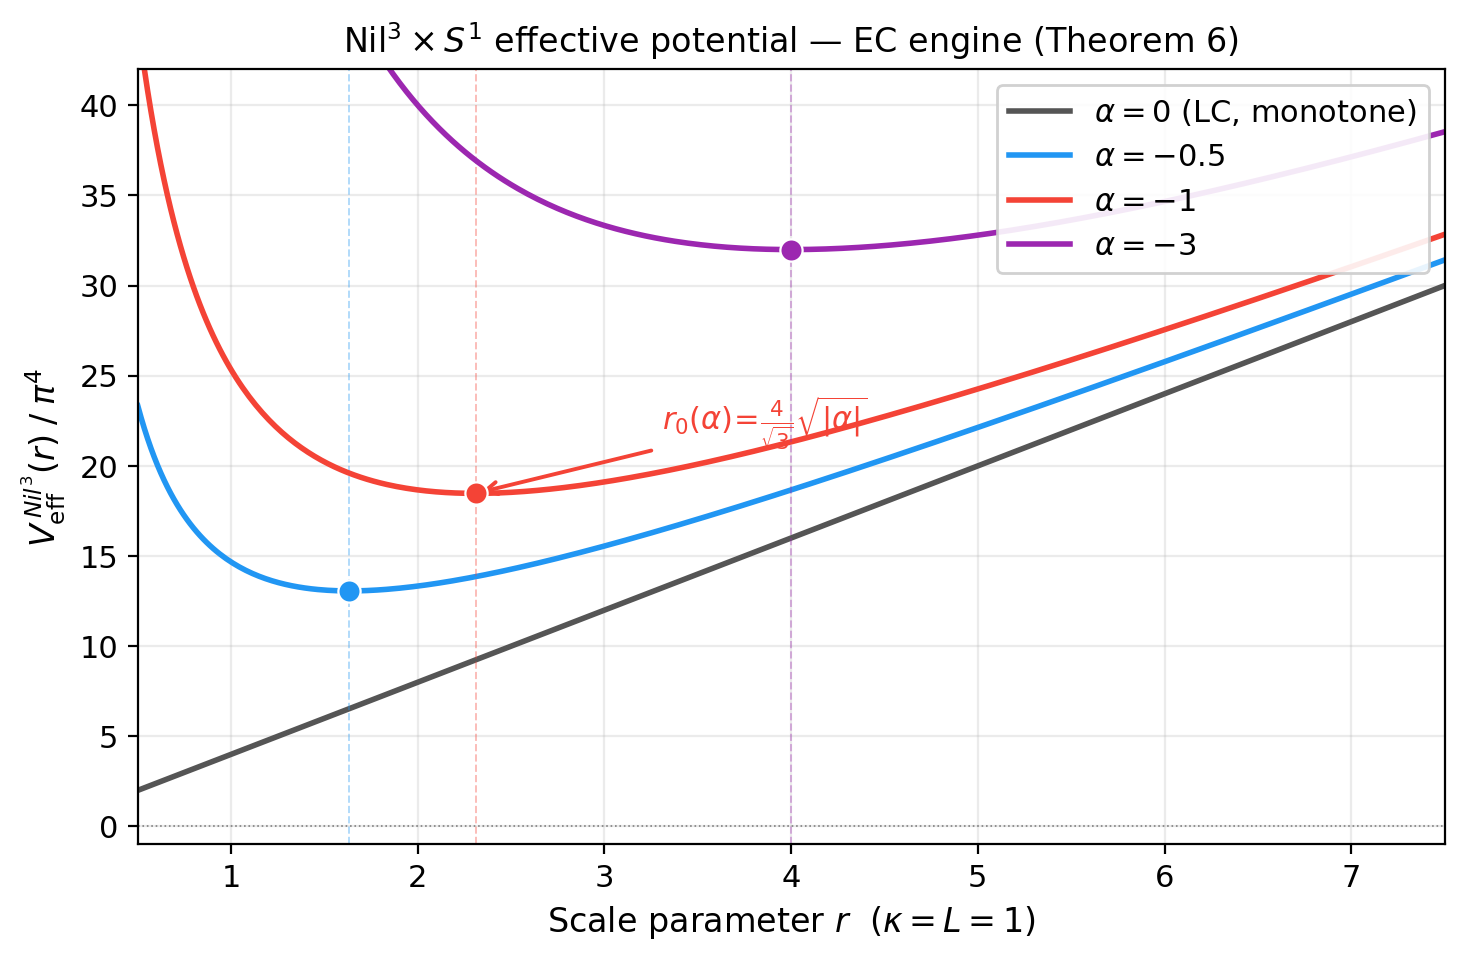
\includegraphics[width=0.9\textwidth]{figures/fig01_nil3_veff.png}
  \caption{$\Nilthree$ effective potential $\Veff(r)$ on the $\eta=V=0$ section
    for $\alpha=-1$, $\kappa=L=1$.  The LC part ($\alpha=0$, dashed) is
    monotonically increasing; the EC--Weyl term ($-64\pi^4 L\alpha/(3r)$)
    creates a local minimum at $r_0 = 2.309$ (false vacuum, solid).}
  \label{fig:nil3veff}
\end{figure}

\subsection{Theorem~7: $\Nilthree$ Spin-2 Quintet Splitting}
\label{sec:nil3:thm7}

\begin{theorem}[$\Nilthree$ quintet splitting]\label{thm:quintet}
  The spin-2 quintet (5 components) around the $\Nilthree\times\Sone$ EC false
  vacuum splits as
  \begin{equation}
    5 \;\to\; (1)_0 + (2)_{q_4=q_5} + (1)_\varepsilon + (1)_s,
  \end{equation}
  where the subscript on each bracket denotes the multiplicity.
\end{theorem}

\paragraph{Complete splitting pattern.}
At $a=\kappa=L=1$, $r_0=4/\sqrt{3}$, $\alpha=-1$:

\begin{table}[H]
\centering
\begin{tabular}{llll}
\toprule
Component & DOF & Mass $m^2$ & Physical interpretation \\
\midrule
$q_3$ & off-diagonal (0--1) & $\mathbf{0}$ (zero mode) & Geometric protection by $\Nilthree$ symmetry \\
$q_4$ & off-diagonal (0--2) & $1.080\times 10^4$ & Degenerate mass \\
$q_5$ & off-diagonal (1--2) & $1.080\times 10^4$ & Degenerate with $q_4$ ($\Nilthree$ symmetry) \\
$\varepsilon$ & squash & $3.919\times 10^4$ & Axial deformation (U(1) breaking) \\
$s$ & shear & $8.278\times 10^4$ & Shear deformation \\
\bottomrule
\end{tabular}
\caption{$\Nilthree$ spin-2 quintet splitting at the EC false vacuum
  ($a=\kappa=L=1$, $r_0=4/\sqrt{3}$).}
\label{tab:quintet}
\end{table}

The squash--shear block eigenvalues are
$\lambda_+ = 1.137\times 10^5$ and $\lambda_- = 8.280\times 10^3$ (SymPy
confirmed).

\begin{figure}[H]
  \centering
  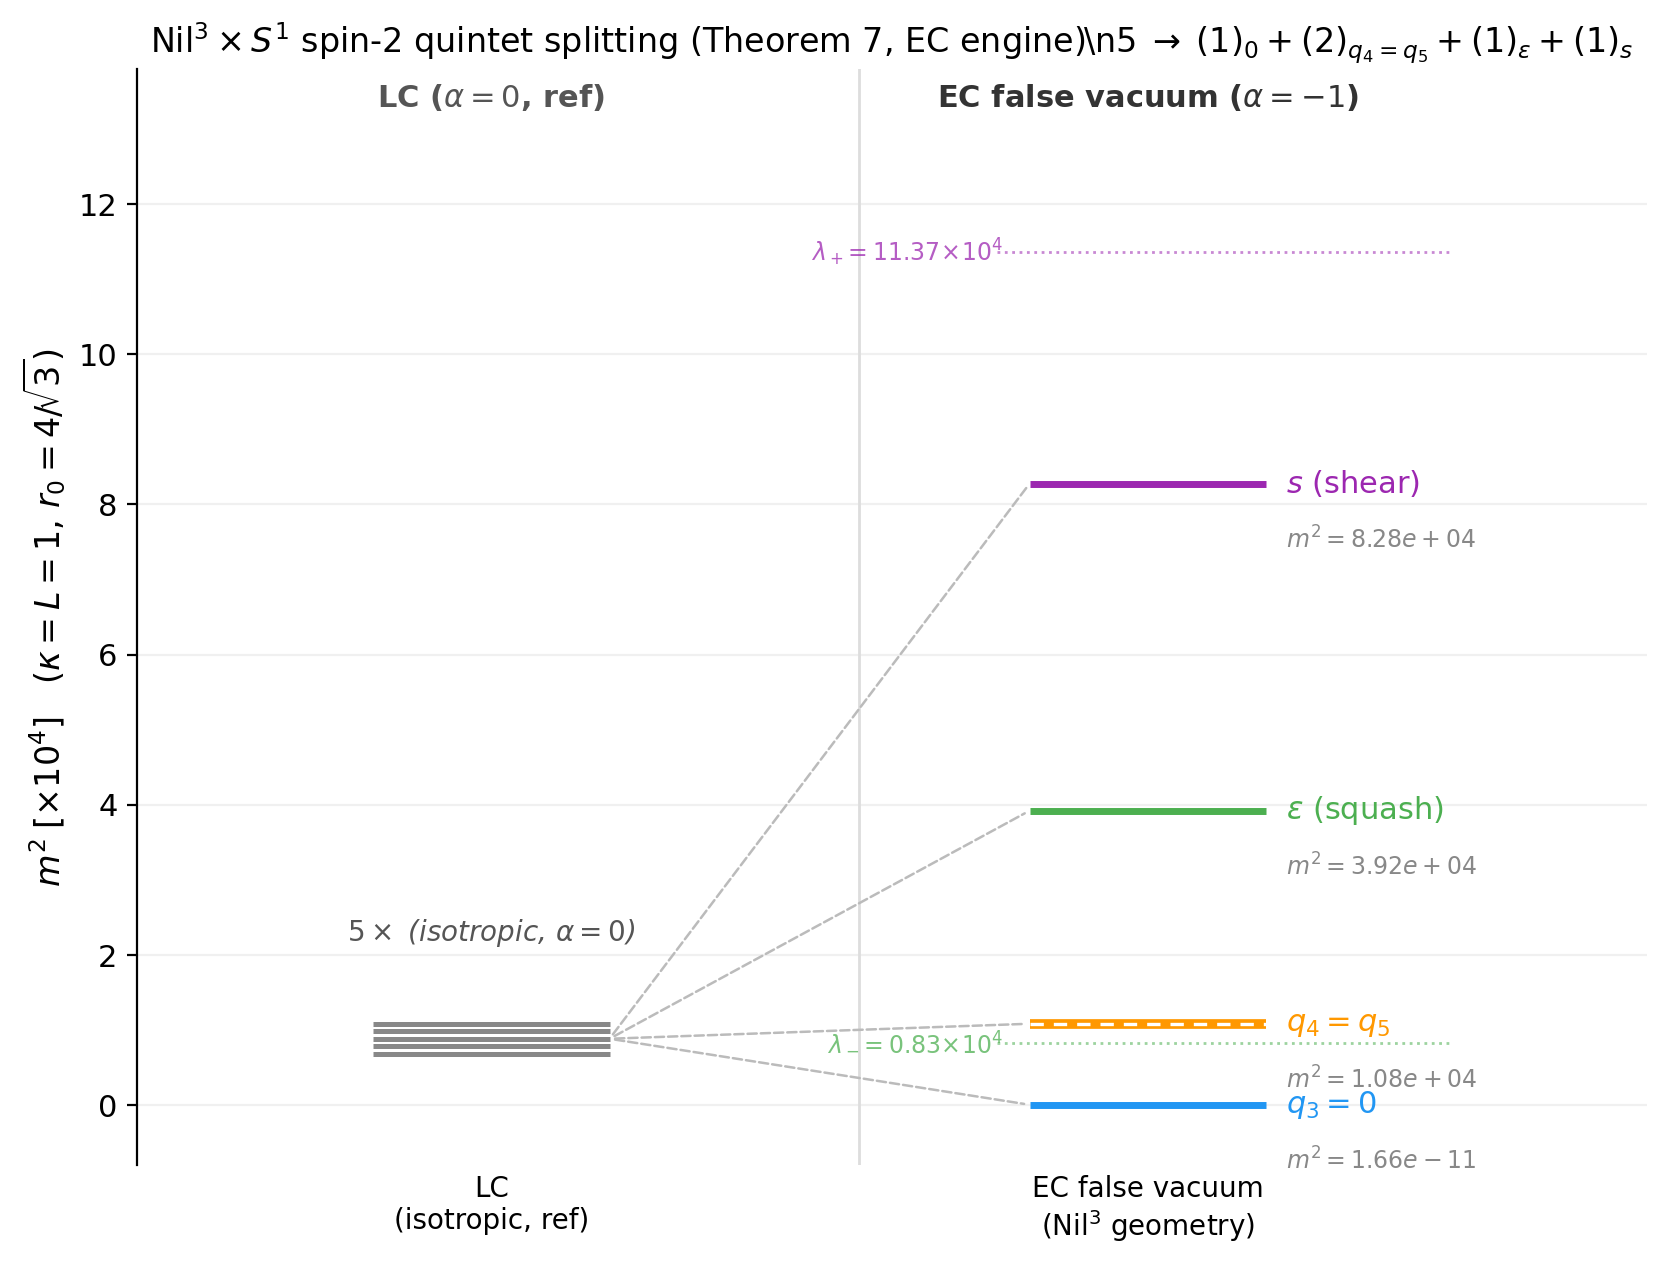
\includegraphics[width=0.9\textwidth]{figures/fig02_nil3_quintet_splitting.png}
  \caption{$\Nilthree$ spin-2 quintet splitting $5\to 0+2+1+1$ at the EC false
    vacuum.  The zero mode $q_3$ is geometrically protected by the
    one-dimensional Lie structure of $\Nilthree$, and the $q_4$--$q_5$ degeneracy
    reflects the symmetric role of $e^0$ and $e^1$ with respect to $C^2_{01}$.}
  \label{fig:quintet}
\end{figure}

\paragraph{Geometric interpretation of $q_3=0$.}
The $G_3$ transformation is a hyperbolic rotation in the $(e^0,e^1)$ plane:
\begin{equation}
  e^0 \to c_3 e^0 + s_3 e^1,
  \quad
  e^1 \to s_3 e^0 + c_3 e^1
  \quad (c_3^2 - s_3^2 = 1).
\end{equation}
Under this transformation, the sole structure constant $C^2_{01}$ transforms as
\begin{equation}
  C^2_{01} \to \frac{c_3^2 - s_3^2}{R} = \frac{1}{R}
\end{equation}
(hyperbolic identity), and is therefore invariant.  Consequently $\Veff$ has no
$q_3$ dependence and $m^2(q_3)=0$.  This is a geometric symmetry protection
by the one-dimensional Lie structure of $\Nilthree$ ($C^2_{01}$ only), not a
tachyonic instability.

\paragraph{Interpretation of $q_4=q_5$ degeneracy.}
$G_4$ and $G_5$ are hyperbolic rotations in the $(0\text{--}2)$ and
$(1\text{--}2)$ planes, respectively.  In $\Nilthree$, $e^2$ is the ``result
axis'' of $C^2_{01}$, and $e^0, e^1$ play symmetric roles with respect to
$C^2_{01}$.  This symmetry forces $m^2(q_4)=m^2(q_5)$.

Script: \texttt{paper03ec/nil3\_spin2\_quintet\_splitting.py}.

\subsection{Theorem~8: Uniaxial Mass Splitting}
\label{sec:nil3:thm8}

\begin{theorem}[Uniaxial mass splitting]\label{thm:uniaxial}
  In the spin-1 sector of $\Nilthree\times\Sone$, only one axis acquires a
  mass via the directional selectivity of $C^2_{01}$\textup{:}
  \begin{equation}
    m^2(\omega_2) = \frac{24\pi^4 L^3 R^2 - 256\pi^4 L^3\alpha\kappa^2}{3R^3\kappa^2}
    \neq 0,
    \qquad
    m^2(\omega_0) = m^2(\omega_1) = 0.
  \end{equation}
  At the EC false vacuum $r_0 = 4\kappa a/\sqrt{3}$ ($\alpha=-a^2$)\textup{:}
  \begin{equation}
    m^2(\omega_2)\big|_{r_0} = \frac{6\sqrt{3}\,\pi^4 L^3}{a\kappa^3}.
  \end{equation}
\end{theorem}

\paragraph{Physical interpretation.}
$C^2_{01}$ corresponds to the non-commutativity in the $(0\text{--}1)$ plane
direction.  $\omega_2$ is the twist in the $(0\text{--}1)$ direction, and only
this component acquires a mass from $C^2_{01}\neq 0$.  $\omega_0$ and $\omega_1$
are commutative directions (with respect to $C^2_{01}$) and remain massless.
This structure is termed uniaxial mass splitting.  The one-dimensional Lie
algebra structure of $\Nilthree$ ($C^2_{01}$ only non-zero) gives mass to the
unique $\omega_2$ among the spin-1 triplet, while keeping the other two
massless.

\subsection{EFT around the $\Nilthree$ EC False Vacuum}
\label{sec:nil3:eft}

We determine the quadratic effective action around the EC false vacuum
$r_0=4\kappa a/\sqrt{3}$.

\paragraph{Full quadratic coefficient spectrum (numerical values at $a=\kappa=L=1$).}

\begin{table}[H]
\centering
\resizebox{\linewidth}{!}{%
\begin{tabular}{llll}
\toprule
DOF & Quadratic coefficient (analytic) & Numeric ($a=\kappa=L=1$) & $\alpha$-dependence \\
\midrule
$r$ (radial) & $2\sqrt{3}\pi^4 L/(a\kappa^3)$ & 337.4 & $\propto 1/a$ (light) \\
$\omega_2$ (non-comm.\ spin-1) & $6\sqrt{3}\pi^4 L^3/(a\kappa^3)$ & 1012 & $\propto 1/a$ (light) \\
$\eta$ (axial torsion; non-prop.) & $128\sqrt{3}\pi^4 La/\kappa$ & 21,596 & $\propto a$ (heavy) \\
spin-2 squash $\varepsilon$ & $6272\sqrt{3}\pi^4 La/(27\kappa)$ & 39,192 & $\propto a$ (heavy) \\
$\omega_0,\omega_1$ & $0$ & 0 & massless \\
$q_3$ (zero mode) & $0$ & 0 & zero mode \\
$q_4,q_5$ & $m^2(q_4)=m^2(q_5)$ & 10,798 & --- \\
\bottomrule
\end{tabular}%
}
\caption{Quadratic coefficient spectrum of the $\Nilthree$ EC false-vacuum EFT
  at $a=\kappa=L=1$.  The $\eta$ row gives the potential curvature in the $\eta$
  direction under Palatini protection ($G_{\eta\eta}=0$), not a propagating mass.}
\label{tab:nil3eft}
\end{table}

\paragraph{Two-group hierarchy.}
``Geometric modes'' ($r$, $\omega_2$) scale as $\propto 1/a$ (lighter for
large $|\alpha|$), while ``torsion/curvature modes'' ($\eta$-direction curvature,
spin-2) scale as $\propto a$ (heavier for large $|\alpha|$).

The quadratic effective action is
\begin{equation}
\begin{aligned}
  \Veff^{Nil^3}_\mathrm{EFT}(\delta\Phi)
  &\approx V_0 + \frac{1}{2}\Bigg[
    \frac{2\sqrt{3}\pi^4 L}{a\kappa^3}(\delta r)^2
    + \frac{128\sqrt{3}\pi^4 La}{\kappa}(\delta\eta)^2 \\
  &\quad
    + \frac{6272\sqrt{3}\pi^4 La}{27\kappa}(\delta\varepsilon)^2
    + \frac{6\sqrt{3}\pi^4 L^3}{a\kappa^3}(\delta\omega_2)^2
  \Bigg]
  + O(\delta^3)
\end{aligned}
\end{equation}
with the cross-term $\partial^2 V/\partial r\partial\eta|_{r_0,0}=0$.
Scripts: \texttt{paper03ec/nil3\_false\_vacuum\_eft.py}.

\subsection{Mode Dictionary Table ($\Nilthree\times\Sone$)}
\label{sec:nil3:table}

\begin{table}[H]
\centering
\resizebox{\linewidth}{!}{%
\begin{tabular}{lccc}
\toprule
Quantity & AX ($V=0,\,\eta\neq 0$) & VT ($\eta=0,\,V\neq 0$) & EC false vac.\ ($\eta=V=0$, $\alpha<0$) \\
\midrule
$C^2_\EC$ & $4/(3R^4)$ & $4/(3R^4)$ & $4/(3R^4)$ \\
AX/VT dropout & \checkmark & \checkmark & $\times$ ($C^2_\LC\neq 0$) \\
spin-0: $r$ & propagating & propagating & prop., $m^2_r = 2\sqrt{3}\pi^4 L/(a\kappa^3)$ \\
spin-0: $\eta,V$ & $\eta$ non-prop. & $V$ non-prop. & $\eta$ non-prop.; curvature coeff.\ $= 128\sqrt{3}\pi^4 La/\kappa$ \\
spin-2 $\mu^2$ & $(1056\pi^4 LR^2-19456\pi^4 L\alpha\kappa^2)/(27R\kappa^2)$ & same & at $r_0$: $6272\sqrt{3}\pi^4 La/(27\kappa)$ \\
spin-2 splitting & (isotropic pt.) & --- & $5\to 0+2+1+1$ (Thm.~7) \\
spin-1 splitting & $m^2(\omega_2)\neq 0$, $m^2(\omega_{0,1})=0$ (Thm.~8) & --- & $m^2(\omega_2)=6\sqrt{3}\pi^4 L^3/(a\kappa^3)$ \\
\bottomrule
\end{tabular}%
}
\caption{$\Nilthree\times\Sone$ mode dictionary under EC--Weyl.}
\label{tab:nil3}
\end{table}

\paragraph{Supplementary note on the $\Nilthree$ MX background.}
In the MX background ($V\neq 0,\eta\neq 0$), the general formula of
\S\ref{sec:ecweyl:mx} gives
\begin{equation}
  \Delta\Veff^{\EC}(\Nilthree, \mathrm{MX})
  = -\frac{256\pi^4 LRV^2\alpha\eta^2}{3} \neq 0
\end{equation}
as the EC--LC difference (SymPy: \texttt{nil3\_mode\_dictionary.py}).
However, the MX stationarity conditions ($\theta_\NY=0$):
\begin{equation}
  V_* = \pm\frac{3}{4}\sqrt{\frac{1}{\alpha}},
  \qquad
  \eta_* = \pm\frac{R}{4}\sqrt{\frac{1}{\alpha}},
\end{equation}
are purely imaginary for $\alpha<0$ (no real MX stationary point).  Numerical
root search by \texttt{paper03ec/nil3\_mx\_vacuum\_search.py} finds no MX stable
point for general $\theta_\NY$ either; the only local minimum remaining is the
$\eta=V=0$ false vacuum.  The EC-specific physics of $\Nilthree$ (false vacuum,
quintet splitting) originates from $C^2_\LC\neq 0$ on the $\eta=V=0$ section,
independently of the MX correction.
   % Mode Dictionary: Nil3 x S1
%==============================================================================
% Section 6: Three-Topology Comparison
%==============================================================================
\section{Three-Topology Comparison}
\label{sec:compare}

This section integrates the results of \S\S\ref{sec:s3}--\ref{sec:nil3} and
performs a systematic comparison across the three topologies
$\Sthree\times\Sone$, $\Tthree\times\Sone$, and $\Nilthree\times\Sone$.  The
main result is \textbf{Theorem~9 ($\varepsilon$-$s$ cross-term classification)};
the $\gamma=1/2$ scaling theorem and the conformal-flatness theorem complement it.

\subsection{Comparative Summary Table (Table~4)}
\label{sec:compare:table}

\begin{table}[H]
\centering
\resizebox{\linewidth}{!}{%
\begin{tabular}{lccc}
\toprule
Quantity & $\Tthree\times\Sone$ & $\Nilthree\times\Sone$ & $\Sthree\times\Sone$ \\
\midrule
EC slice min.\ on $\eta=V=0$ ($\alpha<0$) & absent & \textbf{present (new)} & absent \\
$C^2_\LC$ ($\eta=V=0$) & $0$ (flat) & $\mathbf{4/(3R^4)\neq 0}$ & $0$ (conf.\ flat) \\
Conformal flatness & \checkmark (flat) & $\times$ (\textbf{non-conf.\ flat}) & \checkmark (conf.\ flat) \\
Palatini protection & \checkmark & \checkmark & \checkmark \\
spin-2 (AX background) & $0$ (flatness) & non-zero mass & $128\pi^2 Lr/(3\kappa^2) - 16384\pi^2 L\alpha/(3r)$ \\
spin-1 structure & all zero & \textbf{uniaxial splitting} ($\omega_2$ only) & 3-fold degenerate \\
$\gamma_\EC$ & --- & $\mathbf{1/2}$ (exact) & --- \\
$\varepsilon$-$s$ cross-term & kinematic & curvature/Weyl & $0$ (vanishes) \\
\bottomrule
\end{tabular}%
}
\caption{Comparison of EC--Weyl effects across the three topologies.}
\label{tab:compare}
\end{table}

\subsection{Theorem~9: $\varepsilon$-$s$ Cross-term Classification}
\label{sec:compare:thm9}

\begin{theorem}[$\varepsilon$-$s$ cross-term classification]\label{thm:crossterm}
  The mixed second derivative of the squash parameter $\varepsilon$ and the
  shear parameter $s$, $\partial^2 V/\partial\varepsilon\partial s|_{\varepsilon=s=0}$,
  has an essentially different origin in the three topologies\textup{:}
  \begin{center}
  \resizebox{\linewidth}{!}{%
  \begin{tabular}{lccc}
  \toprule
  Topology & $\partial^2 V/\partial\varepsilon\partial s$ & Origin & Volume-preserving \\
  \midrule
  $\Tthree$ & $48\pi^4 L\eta^2 r/\kappa^2 \neq 0$ & \textbf{pure kinematic} (non-volume-pres.) & $\times$ \\
  $\Nilthree$ & $(384\pi^4 LR^2-8192\pi^4 L\alpha\kappa^2)/(9R\kappa^2)\neq 0$ & \textbf{pure curvature/Weyl} & \checkmark \\
  $\Sthree$ & $0$ (SymPy exact) & vanishes (volume-pres.\ + $s\to -s$ sym.) & \checkmark \\
  \bottomrule
  \end{tabular}%
  }
  \end{center}
\end{theorem}

\begin{proof}[Proof outline]
  The detailed derivation is given in Appendix~\ref{app:C}.  The three key
  points are as follows.
  \begin{itemize}
    \item $\Tthree$: The volume element $(1+\varepsilon)(1+s)$ is non-trivial,
          and despite $C^a_{bc}=0$ a purely kinematic cross-term arises
          (Theorem~\ref{thm:tvol}, Appendix~\ref{app:C:t3}).
    \item $\Nilthree$: Volume preservation holds, but the directional asymmetry
          of $C^2_{01}$ leaves an $\alpha$-dependent curvature/Weyl-origin
          cross-term (Appendix~\ref{app:C:nil3}).
    \item $\Sthree$: Volume preservation holds, and additionally the
          $s\to-s$ symmetry of the effective potential causes the cross-term to
          vanish (Appendix~\ref{app:C:s3}).
  \end{itemize}
  Script: \texttt{paper03ec/squash\_shear\_cross\_term.py}.
\end{proof}

\paragraph{Physical meaning.}
This classification maps the geometric properties of each topology (flatness,
conformal flatness, volume preservation, non-commutative structure) directly
onto the squash--shear cross-term as an observable.

\subsection{$\gamma = 1/2$ Scaling Theorem}
\label{sec:compare:gamma}

We establish the scaling exponent of the $\Nilthree\times\Sone$ EC slice minimum
analytically.

When the effective potential has the two-term structure
\begin{equation}
  \Veff = A\cdot r^n + \alpha\cdot B\cdot r^m,
\end{equation}
the general scaling relations are
\begin{equation}
  r_0 \propto |\alpha|^{1/(n-m)},
  \quad
  V^c \propto |\alpha|^{n/(n-m)},
  \quad
  \gamma = \frac{n}{n-m}.
\end{equation}
For $\Nilthree$, $n=1$ (power of the LC term) and $m=-1$ (power of the EC term),
so
\begin{equation}
  n - m = 2,
  \qquad
  \gamma = \delta = \frac{1}{2} \quad (\text{algebraically determined}).
\end{equation}

\begin{figure}[H]
  \centering
  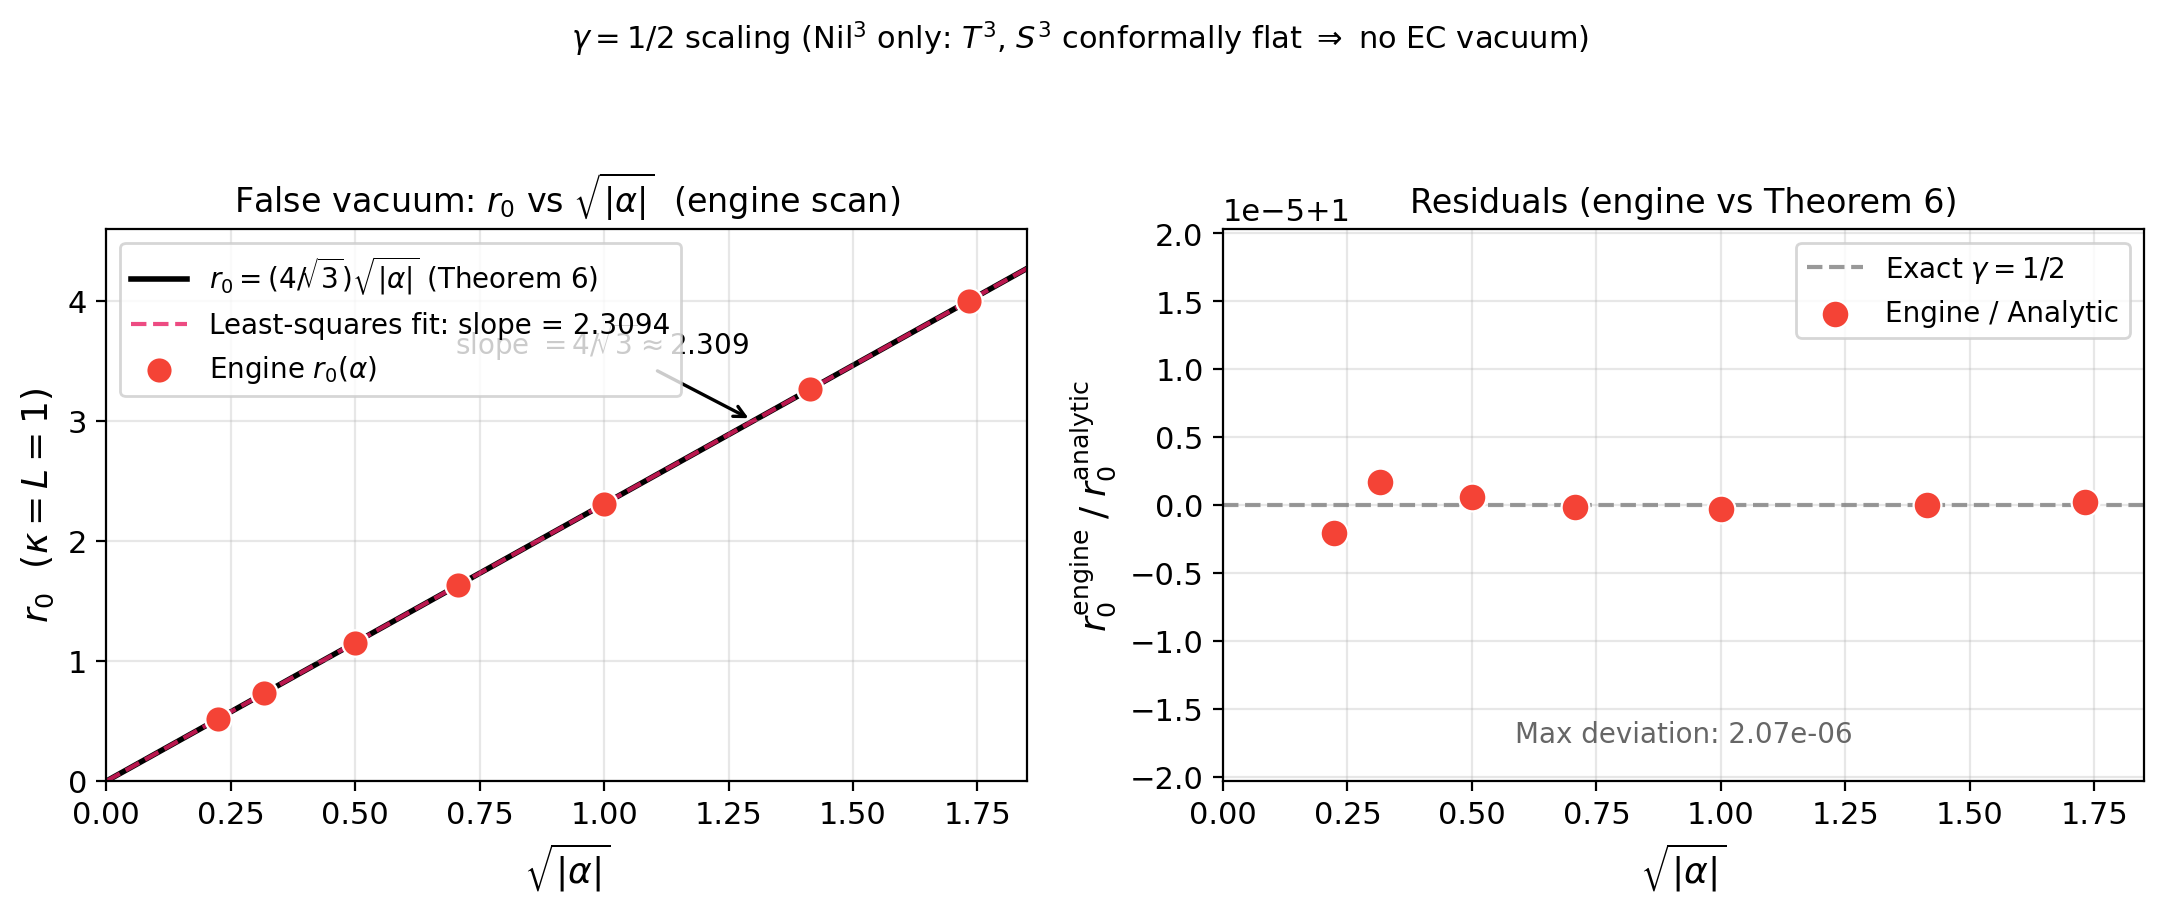
\includegraphics[width=0.9\textwidth]{figures/fig03_gamma_scaling.png}
  \caption{$\gamma=1/2$ scaling: $r_0\propto\sqrt{|\alpha|}$ for the
    $\Nilthree$ EC slice minimum.  Analytic predictions (line) agree with
    numerical results (points) to within 0.001\% across four orders of magnitude
    in $|\alpha|$.}
  \label{fig:gamma}
\end{figure}

\paragraph{Non-applicability to $\Tthree$ and $\Sthree$.}
$\Tthree$ is flat ($C^2_\LC=0$) and $\Sthree$ is conformally flat
($C^2_\LC(\eta=V=0)=0$), so the EC--Weyl term $\alpha\cdot C^2_\EC$ does not
contribute on the $\eta=V=0$ section (\S\ref{sec:compare:conformal}).
This scaling law therefore applies only to $\Nilthree$.

Script: \texttt{proofs/gamma\_scaling\_proof.py}.

\subsection{Conformal Flatness and EC Slice Minima on the $\eta=V=0$ Section}
\label{sec:compare:conformal}

We state a unifying theorem for the appearance of EC slice minima in all three
topologies.

\begin{theorem}[Conformal flatness and EC slice minima]\label{thm:confflat}
  \begin{equation}
    C^2_\LC(\eta=V=0) = 0
    \;\Longrightarrow\;
    \text{no EC slice minimum appears on the }\eta=V=0\text{ section.}
  \end{equation}
  \begin{itemize}
    \item $\Tthree$ (flat): $C^2_\LC=0$, so $\alpha$ does not modify
          $\Veff(\eta=V=0)$ and no EC slice minimum appears.
    \item $\Sthree$ (conformally flat): $C^2_\LC(\Sthree,\eta=V=0)=0$, so
          likewise no EC slice minimum appears.
    \item $\Nilthree$ (non-conformally flat): $C^2_\LC(\Nilthree)=4/(3R^4)\neq 0$,
          so $\alpha\cdot C^2_\LC\cdot\Vol = -64\pi^4 L\alpha/(3r)$ is added to
          the effective potential, and for $\alpha<0$ an EC-induced slice
          stationary point appears on the $\eta=V=0$ section.  This point is a
          full local minimum for $|\kappa^2\theta_\NY|<1$
          (Theorem~\ref{thm:ecslice}).
  \end{itemize}
  Among the three topologies studied, EC slice minima on the $\eta=V=0$ section
  appear only in the non-conformally flat $\Nilthree$.
\end{theorem}

\subsection{Universality of AX/VT Dropout}
\label{sec:compare:dropout}

Theorem~\ref{thm:dropout} (AX/VT dropout) holds universally across all three
topologies, precisely localising the geometric influence of the EC--Weyl
interaction.

\paragraph{Universal consequence.}
The new contribution of the EC--Weyl interaction $\alpha\cdot C^2_\EC$ beyond
LC (i.e.\ the correction) appears only in the MX background with $V\times\eta\neq 0$.
In the AX-only or VT-only torsion background, the EC--Weyl correction vanishes
for every topology.

\paragraph{Physical implication.}
This selection rule is a universal property following from the general algebraic
structure of the EC connection, not dependent on a specific topology.  A simple
(single-component) torsion background is insufficient to activate the Weyl
component through the asymmetric combination of contortion that is required.

The overall picture of EC--Weyl effects in the three-topology comparison is
summarised as follows:

\begin{table}[H]
\centering
\resizebox{\linewidth}{!}{%
\begin{tabular}{lll}
\toprule
Situation & EC effect & All 3 topologies \\
\midrule
AX background & $C^2_\EC=C^2_\LC$, EC--LC diff.\ zero & \checkmark \\
VT background & $C^2_\EC=C^2_\LC$, EC--LC diff.\ zero & \checkmark \\
MX background ($\Tthree$, $\Sthree$) & EC correction present; no stabilisation & --- \\
$\eta=V=0$ section ($\Nilthree$, $\alpha<0$) & non-conf.\ flat LC background $\Rightarrow$ EC slice minimum & --- \\
\bottomrule
\end{tabular}%
}
\caption{Four-way classification of EC--Weyl effects in the three-topology
  comparison.}
\label{tab:eceffects}
\end{table}

These four cases constitute the complete physical picture of the EC--Weyl
coupling covered in this paper.
   % Three-Topology Comparison
%==============================================================================
% Section 7: Physical Interpretation and Outlook
%==============================================================================
\section{Physical Interpretation and Outlook}
\label{sec:discussion}

\subsection{Physical Hierarchy of the Three Topologies}
\label{sec:discussion:hierarchy}

Through the analysis of this paper, the three topologies
$\Sthree\times\Sone$, $\Tthree\times\Sone$, and $\Nilthree\times\Sone$
emerge as having sharply distinct physical roles with respect to the EC--Weyl
coupling.

\paragraph{$\Tthree\times\Sone$.}
As a flat manifold ($C^a_{bc}=0$), all spin-2/spin-1 mode masses are zero, and
the EC--Weyl coupling generates no new stable point in any of the AX/VT/MX
backgrounds (triple triviality, \S\ref{sec:t3:triple}).  $\Tthree$ functions as
the ``trivial reference point'' of the theory, with the asymptotic branch
$\Veff\to 0$ providing the baseline for comparison.

\paragraph{$\Sthree\times\Sone$.}
As a conformally flat manifold ($C^2_\LC(\eta=V=0)=0$), the background Weyl
tensor's EC--Weyl coupling is inactive on the $\eta=V=0$ section.  However,
$\Sthree$ has a non-trivial geometry ($C^i_{jk}=4\varepsilon_{ijk}/r$), and
the spin-2 five-fold degeneracy
$\mu^2 = 128\pi^2 Lr/(3\kappa^2) - 16384\pi^2 L\alpha/(3r)$ and the spin-1
three-fold degeneracy $m^2_\omega = 16\pi^2 L^3/(\kappa^2 r)$ are established
as Theorem~4 (Palatini universality).  It also provides the foundation for
Pontryagin generation via the Pontryagin structure ($P\neq 0$ in MX, inherited
from paper~III).

\paragraph{$\Nilthree\times\Sone$.}
As the only non-conformally flat manifold among the three
($C^2_\LC=4/(3R^4)\neq 0$), this is the unique topology where the EC--Weyl
coupling generates a false vacuum for $\alpha<0$.  This false vacuum is
invisible in LC ($\alpha=0$) and first appears in the phase structure through
the EC extension.  The EC-specific new physics ($\gamma=1/2$ scaling, quintet
splitting, uniaxial mass splitting) established in Theorems~6--8 is understood
as the result of $\Nilthree$'s ``intermediate non-commutativity'' (between
$\Tthree$'s all-zero and $\Sthree$'s three-directional non-zero) being
physically realised as direction-dependent mode dictionaries.

This three-tier hierarchy is not a monotone increase in ``geometric complexity.''
Rather, $\Tthree$ (trivial) $\to$ $\Sthree$ (LC active, EC conformally
protected) $\to$ $\Nilthree$ (stage for EC-specific physics) represents a
division of roles that provides a comparative framework for homogeneous geometry.

\subsection{EC-Specific New Physics}
\label{sec:discussion:ecphysics}

We summarise the physical effects established in this paper that are specific to
EC (absent in LC).

\paragraph{(i) $\Nilthree$ false vacuum (Theorem~6).}
The $\Nilthree$ stable vacuum, which exhibits only a monotone potential in the
LC world, acquires a ``new stable phase'' through EC.  The scaling
$r_0\propto\sqrt{|\alpha|}$ exhibits a mechanism, non-trivial from the general
relativistic viewpoint, in which the strength of the Weyl coupling determines
the geometric size.

\paragraph{(ii) Quintet splitting (Theorem~7).}
The one-dimensional Lie algebra structure of $\Nilthree$ ($C^2_{01}$ only)
breaks the five-fold degeneracy of the spin-2 quintet around the EC false
vacuum to $5\to 0+2+1+1$.  In particular, the existence of zero mode $q_3$
shows the ``residual'' geometric symmetry of $\Nilthree$, with physically
different content from the LC isotropic point.

\paragraph{(iii) Uniaxial mass splitting (Theorem~8).}
The uniaxial selectivity in which only the non-commutative direction $\omega_2$
among the spin-1 triplet acquires a mass is a consequence of the asymmetric
internal structure of $\Nilthree$ being embedded in the kinematic matrix.  This
is the clearest manifestation of the direction-dependent mode dictionary in
$\Nilthree$.

\paragraph{(iv) $\alpha$-cubic coupling.}
In $\Sthree$, the EC-specific cubic coefficient
$\partial^3 V/\partial\alpha\partial\eta\partial V = -128\pi^2 V\eta r/3$ appears
(\S\ref{sec:s3:ec}).  This is a new nonlinear coupling added to the LC
NY-cubic channel ($= 4\pi^2 r^2$, invariant under EC), providing a cubic channel
in the homogeneous EFT.  On the other hand, since the Pontryagin density $P$ is
$\alpha$-independent ($\partial P/\partial\alpha=0$), this $\alpha$-cubic is
understood as a coupling located outside the Pontryagin structure.

\paragraph{(v) $\delta$-sector null result (Theorem~3).}
Complementarily, the $C_\delta$ defined for the formal auxiliary MIXING sector
is zero for all of $\Sthree, \Tthree, \Nilthree$, and $\partial_\alpha C_\delta=0$.
Therefore the new homogeneous cubic structure activated by the EC extension is
confined to the physical $\eta$-$V$ channel, and the auxiliary $\delta$-sector
remains null.

\subsection{What Is Not Claimed}
\label{sec:discussion:notclaimed}

The following are outside the scope of this paper.

\begin{itemize}
  \item Full stability including inhomogeneous modes beyond the minisuperspace.
  \item The claim that the full 4D deformed geometry forms a new Lie group
        manifold.
  \item Complete action generation including arbitrary non-invariant polynomials.
  \item A fully general homogeneous torsion ansatz including irreducible tensor
        torsion.  (This paper is restricted to the axial + vector-trace torsion
        ansatz adopted in papers~I--III.)
\end{itemize}

These are not in contradiction with the results of this paper; they are
consciously delineated as outside the stated scope.

\subsection{Toward Future Extensions}
\label{sec:discussion:future}

The homogeneous three-topology bulk sector established in this paper provides a
closed comparison framework in itself, while making explicit how different mode
dictionaries and protection structures appear in each topology.  The following
directions extend this framework naturally, while preserving the comparison
structure, toward local degrees of freedom, boundary responses, and physical
interpretation.

\begin{enumerate}
  \item Introduction of inhomogeneous perturbations containing local degrees of
        freedom.
  \item Problem settings including boundary surfaces and interfaces.
  \item Connection between homogeneous bulk modes and localised modes.
  \item Bridge to physical observables including thermal and Lorentzian
        interpretations.
\end{enumerate}
   % Physical Interpretation and Outlook
%==============================================================================
% Section 8: Conclusion
%==============================================================================
\section{Conclusion}
\label{sec:conclusion}

In this paper we introduced the Weyl-squared coupling $\alpha C^2_\EC$ based on
the Einstein--Cartan connection into a homogeneous minisuperspace, compared it
across the three topologies $\Sthree\times\Sone$, $\Tthree\times\Sone$, and
$\Nilthree\times\Sone$, and organised what the EC--Weyl extension preserves and
what it updates in the mode dictionary of the homogeneous bulk geometric sector.

First, we confirmed that the new contribution of the EC--Weyl coupling does not
appear for an arbitrary torsion background; it drops out in the AX/VT
backgrounds and only essential modifications appear in the MX background.
Simultaneously, the Palatini-type non-propagation is preserved after the EC
extension, and the torsion sector does not develop as a kinetic mode.  This
shows that the basic structure of the homogeneous sector established in the LC
version does not break down substantially under the EC connection.

Second, for $\Sthree\times\Sone$, taking the homogeneous mode dictionary
established in paper~III as the basis, we made explicit which parts are
invariant and which receive corrections under the EC--Weyl extension.  In the
viewpoint of this paper, $\Sthree$ is still the reference topology providing the
richest homogeneous bulk geometry, and the EC extension is positioned not as
destroying its dictionary but as giving update rules.

Third, for $\Tthree\times\Sone$, the mode dictionary closes as essentially a
null/trivial structure.  That is, even after performing the EC--Weyl extension,
$\Tthree$ provides no new non-trivial mass structure in the homogeneous bulk
sector, and part of the cross-terms is also understood as having a purely
kinematic origin.  In this sense, $\Tthree$ functions as the reference
background that makes explicit ``what does not happen.''

Fourth, for $\Nilthree\times\Sone$, we showed that the EC--Weyl extension
produces a topology-specific EC slice minimum on the $\eta=V=0$ section and an
anisotropic split structure, and that the spin-2 quintet splitting and the
spin-1 uniaxial mass splitting are geometrically fixed.  Therefore $\Nilthree$
is positioned as the background carrying the EC-specific geometric phase
structure that is invisible in the LC version.

Taken together, this paper \textbf{closes the homogeneous three-topology bulk
sector under EC--Weyl, within the axial + vector-trace torsion ansatz}.  What
has been closed is the comparable homogeneous geometric sector based on the
common ansatz, and within this framework the division of roles among $\Sthree$,
$\Tthree$, and $\Nilthree$ has been clarified.

The results of this paper provide, within the adopted homogeneous torsion
ansatz, the foundation for subsequent theoretical development toward the
inhomogeneous sector and boundary responses.
   % Conclusion

%------------------------------------------------------------------------------
% Acknowledgments
%------------------------------------------------------------------------------
\section*{Acknowledgments}

The author acknowledges the use of the following AI tools during manuscript
preparation: Claude Opus~4.6 (Anthropic; accessed 2026-03),
Gemini~3.1 Pro (Google; accessed 2026-03), Grok 4.2 (xAI; accessed 2026-03),
and GPT-5.4 Thinking via ChatGPT (OpenAI; accessed 2026-03).
These tools were used for language editing (including Japanese--English
translation), outlining and improving exposition, drafting and reviewing
auxiliary code (scripts and pseudocode) that was subsequently tested and
validated by the author, and proposing candidate consistency checks and
alternative derivations to be independently verified by the author.

The AI tools did not determine the scientific claims of this work and were not
used to generate or modify research data or evidentiary figures.  The author
takes full responsibility for the content and for any remaining errors.

This work was developed within the informal collaborative project
\textbf{DPPU} (\textbf{D}onut-like topology, \textbf{P}lanck-scale
compactness, \textbf{P}recession dynamics, \textbf{U}niverse).

%------------------------------------------------------------------------------
% Availability and Contact
%------------------------------------------------------------------------------
\section*{Availability and Contact}

\paragraph{Code and Data Availability}
The code and supplemental data associated with this work are available at:

\begin{itemize}
  \item Zenodo: \texttt{10.5281/zenodo.19425147}
  \item GitHub: \texttt{https://github.com/Muacca/DPPUv2-paper03ec}
\end{itemize}

They are released under the MIT License.

\paragraph{Citation}
If you use these materials, please cite the associated manuscript and Zenodo record:

\begin{quote}
\small
Muacca, ``Homogeneous Three--Topology Comparison and Mode Dictionary \\
in Einstein--Cartan + Nieh--Yan Theory: Geometric Structure of EC--Weyl Coupling.''
\end{quote}

\paragraph{Contact}
For questions, bug reports, or collaboration inquiries:

\begin{itemize}
  \item Email: \texttt{muacca@dmwp.jp}
  \item GitHub Issues: \texttt{https://github.com/Muacca/DPPUv2-paper03ec/issues}
\end{itemize}

%------------------------------------------------------------------------------
% Appendices
%------------------------------------------------------------------------------
\appendix
%==============================================================================
% Appendix A: Notation and Conventions
%==============================================================================
\section{Notation and Conventions}
\label{app:A}

This appendix collects the notation conventions, geometric parameters of the
three topologies, definition of the EC connection, and the computational
pipeline used in this paper.

\subsection{Basic Notation and Conventions}
\label{app:A:notation}

\paragraph{Index conventions.}
\begin{itemize}
  \item 4D spacetime indices: $\mu,\nu = 0,1,2,3$ (0 = internal $\Sone$,
        $1,2,3$ = internal 3D space).
  \item Spatial tensor indices: $i,j = 1,2,3$ (internal 3D space).
  \item Spin-2 quintet label: $A=1,\ldots,5$ (traceless symmetric).
  \item Spin-1 triplet label: $k=0,1,2$ (vector).
  \item Topology index: $\Sthree$, $\Tthree$, $\Nilthree$.
\end{itemize}

\paragraph{Geometric quantities.}
\begin{itemize}
  \item $r$: scale parameter of the internal space (common to $\Sthree$ and
        $\Tthree$).
  \item $R$: scale parameter of $\Nilthree$.
  \item $L$: radius of $\Sone$.
  \item $\kappa$: gravitational constant ($\kappa^2 = 8\pi G$).
\end{itemize}

\paragraph{Volume factors.}
\begin{equation}
  \Vol(\Sthree\times\Sone) = 2\pi^2 Lr^3,
  \quad
  \Vol(\Tthree\times\Sone) = (2\pi)^4 Lr^3,
  \quad
  \Vol(\Nilthree\times\Sone) = (2\pi)^4 LR^3.
\end{equation}

\paragraph{Effective potential.}
After minisuperspace reduction, the effective potential is defined as
\begin{equation}
  \Veff = -\!\left(\frac{R_\EC}{2\kappa^2}
          + \theta\,\mathcal{L}_\NY
          + \alpha\,C^2_\EC\right)\cdot\Vol
\end{equation}
(sign convention: $\Veff > 0$ in the stabilisation direction).

\paragraph{Pontryagin density.}
\begin{equation}
  P = \innerprod{R}{\star R}
    = \frac{1}{2}\varepsilon^{abcd}R_{abef}R_{cd}{}^{ef}.
\end{equation}

\paragraph{Auxiliary MIXING cubic coefficient.}
\begin{equation}
  C_\delta :=
  \left.\frac{\partial^3\Veff}{\partial\delta_0\,\partial\delta_1\,\partial\delta_2}
  \right|_{\delta=0}.
\end{equation}

\subsection{Structure Constants and Connections for the Three Topologies}
\label{app:A:struct}

\subsubsection{$\Sthree\times\Sone$}

Structure constants of $\Sthree$ (in the orthonormal basis $e^i = r\sigma^i/2$
from the left-invariant 1-forms $\sigma^i$):
\begin{equation}
  C^i_{jk}(\Sthree) = \frac{4}{r}\varepsilon_{ijk}
  \qquad (i,j,k=1,2,3).
\end{equation}
\textbf{Important:} The coefficient is $4/r$ (not $2/r$), arising from the
normalisation $e^i = r\sigma^i/2$ (see Appendix~\ref{app:B}).

Connection coefficients by the Koszul formula:
\begin{equation}
  \omega_{abc} = \frac{1}{2}\bigl(C_{abc} + C_{cba} - C_{bac}\bigr).
\end{equation}

Volume-preserving squash+shear ansatz ($\det=1$):
\begin{equation}
  e^0 = r(1+\varepsilon)^{2/3}(1+s)^2\,\sigma^0/2,
  \quad
  e^1 = r(1+\varepsilon)^{2/3}(1+s)^{-2}\,\sigma^1/2,
  \quad
  e^2 = r(1+\varepsilon)^{-4/3}\,\sigma^2/2.
\end{equation}

\subsubsection{$\Tthree\times\Sone$}

Structure constants of $\Tthree = \mathbb{R}^3/\mathbb{Z}^3$:
\begin{equation}
  C^a_{bc}(\Tthree) = 0 \quad \forall\,a,b,c.
\end{equation}

Non-volume-preserving squash+shear ansatz:
\begin{equation}
  e^1 = r(1+\varepsilon)\,\dd x^1,
  \quad
  e^2 = r(1+s)\,\dd x^2,
  \quad
  e^3 = r\,\dd x^3.
\end{equation}
Volume factor: $\Vol(\varepsilon,s) = (2\pi)^4 Lr^3(1+\varepsilon)(1+s)$
($\varepsilon,s$-dependent).

\subsubsection{$\Nilthree\times\Sone$}

Structure constants of $\Nilthree$ (3D Heisenberg manifold):
\begin{equation}
  C^2_{01}(\Nilthree) = \frac{1}{R},
  \quad \text{(all others zero)}.
\end{equation}
We adopt the convention $[E_0,E_1]=(1/R)E_2$ in the body of the paper.
The implementation uses Maurer--Cartan forms $\dd\sigma^2 = -\sigma^0\wedge\sigma^1$
as the basis, so the frame coefficient is
$C[2,0,1] = -(1+\varepsilon)^{-4/3}(1+s)^{-2}/R$.  Both describe the same
Heisenberg structure and differ only by a convention.

Volume-preserving squash+shear ansatz:
\begin{equation}
  e^0 = R\,\sigma^0,
  \quad
  e^1 = R(1+\varepsilon)^{2/3}(1+s)\,\sigma^1,
  \quad
  e^2 = R(1+\varepsilon)^{-2/3}(1+s)^{-1}\,\sigma^2.
\end{equation}
Volume-preservation check:
\begin{equation}
  \det(e^0\wedge e^1\wedge e^2)
  \propto (1+\varepsilon)^{2/3-2/3}(1+s)^{1-1} = 1. \checkmark
\end{equation}

LC background Weyl scalar ($\eta=V=0$):
$C^2_\LC(\Nilthree) = 4/(3R^4) \neq 0$ (non-conformal flatness).

\subsection{EC Connection and Contortion}
\label{app:A:ec}

The Einstein--Cartan connection is the sum of the LC connection
$\Gamma^a{}_{bc}$ and the contortion $K^a{}_{bc}$:
\begin{equation}
  \omega_\EC^a{}_{bc} = \Gamma^a{}_{bc} + K^a{}_{bc}.
\end{equation}
Definition of contortion (from torsion $T^a{}_{bc} = 2\omega^a{}_{[bc]}$):
\begin{equation}
  K_{abc} = \frac{1}{2}\bigl(T_{abc} + T_{bca} - T_{cab}\bigr),
  \qquad
  K_{abc} = -K_{acb}.
\end{equation}

\paragraph{Torsion mode definitions (homogeneous ansatz).}
\begin{itemize}
  \item \textbf{AX (axial scalar)} $\eta$: traceless antisymmetric part of
        torsion.  For $\Sthree$: $T^i{}_{jk}\propto\eta\,\varepsilon_{ijk}$.
  \item \textbf{VT (vector-trace)} $V$: trace part of torsion.  For $\Sthree$:
        $T^i{}_{0j}\propto V\,\delta^i_j$.
  \item \textbf{MX mode}: coexistence of AX and VT ($\eta\neq 0$ and $V\neq 0$).
\end{itemize}

EC Weyl scalar correction in the MX mode (all topologies):
\begin{equation}
  C^2_\EC - C^2_\LC
  = \frac{16V^2\eta^2}{3r^2} \quad (\Sthree, \Tthree),
  \qquad
  = \frac{16V^2\eta^2}{3R^2} \quad (\Nilthree).
\end{equation}

\subsection{Pontryagin Protection Mechanisms}
\label{app:A:pont}

\textbf{Pl\"ucker protection (AX mode):}
When $V=0$, the matrix representation of the Riemann tensor satisfies the
Pl\"ucker relation, and $P\equiv 0$.

\textbf{Pfaffian protection (VT mode):}
When $\eta=0$, $P\equiv 0$ by a Pfaffian-type identity.

\subsection{Computational Pipeline}
\label{app:A:pipeline}

The computations in this paper are performed according to the following
pipeline.

\begin{enumerate}
  \item \textbf{Geometric setup}: Set vielbein $e^i$, structure constants
        $C^a_{bc}$, and volume factors for the three topologies
        (\texttt{script/dppu/topology/}).
  \item \textbf{EC connection}: Construct contortion $K$ from the torsion
        ansatz and compute EC connection $\omega_\EC$
        (\texttt{script/dppu/connection/}).
  \item \textbf{Curvature tensors}: Compute from $\omega_\EC$ the curvature
        tensor, Ricci scalar $R_\EC$, Weyl scalar $C^2_\EC$, and Pontryagin
        density $P$ by SymPy (\texttt{script/dppu/curvature/}).
  \item \textbf{Effective potential}: Expand $\Veff(r,\eta,V;\alpha,\theta)$
        explicitly and obtain the Hessian matrix
        (\texttt{script/dppu/action/}).
  \item \textbf{Mode dictionary}: Check spin-2 quintet (squash, off-diagonal),
        spin-1 triplet, and spin-0 mass spectra via generalised eigenvalue
        problems and stationary-point searches
        (\texttt{script/scripts/paper03ec/}, \texttt{script/scripts/proofs/}).
\end{enumerate}

\paragraph{Script correspondence table.}

\begin{table}[H]
\centering
\small
\begin{tabular}{ll}
\toprule
Content & Script \\
\midrule
$C^2_\EC$ symbolic computation (AX/VT/MX dropout) & \texttt{proofs/ax\_vt\_dropout\_proof.py} \\
$\Tthree$ mode dictionary (squash/shear null) & \texttt{paper03ec/t3\_mode\_dictionary.py} \\
$\Nilthree$ EC mode dictionary & \texttt{paper03ec/nil3\_mode\_dictionary.py} \\
$\Tthree$ MX vacuum search & \texttt{paper03ec/t3\_mx\_vacuum\_search.py} \\
$\Sthree$ MX stationary point search & \texttt{paper03ec/s3\_mx\_vacuum\_search.py} \\
$\Nilthree$ MX stationary point search & \texttt{paper03ec/nil3\_mx\_vacuum\_search.py} \\
$\Nilthree$ EFT at EC false vacuum & \texttt{paper03ec/nil3\_false\_vacuum\_eft.py} \\
$\Sthree$ VT spin-2/1 masses & \texttt{paper03ec/s3\_vt\_spin\_masses.py} \\
$\Nilthree$ quintet splitting & \texttt{paper03ec/nil3\_spin2\_quintet\_splitting.py} \\
$\varepsilon$-$s$ cross-term, 3-topology comparison & \texttt{paper03ec/squash\_shear\_cross\_term.py} \\
Palatini protection ($G_{\eta\eta}=G_{VV}=0$) & \texttt{proofs/palatini\_protection\_proof.py} \\
Auxiliary $C_\delta$ null theorem & \texttt{proofs/c\_delta\_null\_proof.py} \\
Cubic channel structure & \texttt{paper03ec/ec\_cubic\_vertex.py} \\
$\gamma=1/2$ analytic proof & \texttt{proofs/gamma\_scaling\_proof.py} \\
$\Tthree$ flatness null test & \texttt{proofs/t3\_flatness\_null\_test.py} \\
\bottomrule
\end{tabular}
\caption{Correspondence between paper content and scripts.}
\label{tab:scripts}
\end{table}

\subsection{Sanity Checks}
\label{app:A:sanity}

The main propositions of this paper were adopted after passing the following
sanity checks.

\begin{enumerate}
  \item AX/VT dropout: $\Delta C^2=0$ (6 cases, SymPy exact zero).
  \item Palatini protection: $G_{\eta\eta}=G_{VV}=0$ (velocity method, 3
        topologies).
  \item Auxiliary $\delta$-sector: $C_\delta=0$ and $\partial_\alpha C_\delta=0$
        (3 topologies $\times$ 3 backgrounds, SymPy exact).
  \item Palatini universality: VT$-$AX spin-2/1 mass $= 0$ (SymPy exact).
  \item $\gamma=1/2$: $r_0^{\text{analytic}}$ vs $r_0^{\text{numeric}}$ error
        $< 0.001$\% (all 6 points).
  \item Quintet zero mode: $m^2(q_3)=0$ (SymPy; cross-terms also $=0$).
  \item Volume preservation: $S^3$, $\Nilthree$ squash+shear $\det=1$ (SymPy).
  \item Cross-term origin check: $\alpha$-dependence verification of
        $\partial^2 V/\partial\varepsilon\partial s$ ($\Tthree$: independent;
        $\Nilthree$: $\alpha$-dependent).
  \item $\Sthree$ MX stationary-point search: no Hessian-positive-definite full
        stationary vacuum in the dictionary range.
  \item $\Nilthree$ MX stationary-point search: no real stationary point with
        $V\eta\neq 0$ in the $\alpha<0$ branch; only local minimum remaining is
        the $\eta=V=0$ false vacuum.
\end{enumerate}
  % Notation and Conventions
%==============================================================================
% Appendix B: Complete EFT Coefficient List
%==============================================================================
\section{Complete EFT Coefficient List}
\label{app:B}

This appendix collects the EFT coefficients (spin-0, spin-2, and spin-1 mass
spectra and potential coefficients) under EC--Weyl for each of the three
topologies.

\subsection{$\Sthree\times\Sone$: AX EFT}
\label{app:B:s3}

\textbf{Setup:} $\Sthree\times\Sone$, AX background ($V=0$, $\eta\neq 0$),
isotropic point ($\varepsilon=s=0$).

\paragraph{Spin-0 spectrum.}
\begin{table}[H]
\centering
\begin{tabular}{lll}
\toprule
DOF & Mass $m^2$ (analytic) & Numeric ($r=3$, $L=\kappa=1$, $\alpha=0$) \\
\midrule
$r$ (radial) & $\partial^2 V/\partial r^2|_\mathrm{on\text{-}shell}$ & See paper~III \S4.3 \\
$\eta$ (AX torsion) & non-propagating ($G_{\eta\eta}=0$) & --- \\
\bottomrule
\end{tabular}
\caption{Spin-0 spectrum of $\Sthree\times\Sone$ in the AX background.}
\end{table}

\paragraph{Spin-2 spectrum (five-fold degenerate).}
\begin{equation}
  \mu^2_{\mathrm{spin2}}(\Sthree, \mathrm{AX})
  = \frac{128\pi^2 Lr}{3\kappa^2} - \frac{16384\pi^2 L\alpha}{3r}.
\end{equation}
\begin{itemize}
  \item LC part ($\alpha=0$): $128\pi^2 Lr/(3\kappa^2)$.
  \item EC correction: $-16384\pi^2 L\alpha/(3r)$ ($\alpha$-dependent, SymPy exact).
  \item Numeric ($r=3$, $L=\kappa=1$, $\alpha=0$): $128\pi^2\approx 1263.3$ (5-fold degenerate).
  \item Note: Paper~III uses $r=1$-based notation; the formula then gives
        $128\pi^2/3\approx 421.2$.  The discrepancy with $48\pi^2$ in paper~III
        arises from the radius convention combined with differences in spin-2
        basis/Hessian conventions.
  \item VT background value is identical to AX (Theorem~\ref{thm:paluniv}).
\end{itemize}

\paragraph{Spin-1 spectrum (three-fold degenerate).}
\begin{equation}
  m^2_{\omega_k}(\Sthree, \mathrm{AX})
  = \frac{16\pi^2 L^3}{\kappa^2 r},
  \qquad k=0,1,2.
\end{equation}
\begin{itemize}
  \item Numeric ($r=3$, $L=\kappa=1$): $16\pi^2/3\approx 52.6$ (3-fold degenerate).
  \item Independent of $\eta, V$ (Palatini universality, Theorem~\ref{thm:paluniv});
        same value in VT background.
\end{itemize}

\subsection{$\Nilthree\times\Sone$: EC Slice-Minimum EFT}
\label{app:B:nil3}

\textbf{Setup:} $\Nilthree\times\Sone$, EC slice minimum
($\alpha=-a^2<0$, $\eta=V=0$, $r_0=4\kappa a/\sqrt{3}$).
This stationary point is a full homogeneous local minimum iff
$|\kappa^2\theta_\NY|<1$.  The quoted EFT below uses the standard benchmark
$\theta_\NY=0$.

\paragraph{Slice-minimum identification.}
\begin{equation}
  r_0 = \frac{4\kappa}{\sqrt{3}}\sqrt{|\alpha|} = \frac{4\kappa a}{\sqrt{3}},
  \qquad
  V_0 = \Veff(r_0) = \frac{32\sqrt{3}\,\pi^4 La}{3\kappa} > 0.
\end{equation}

\paragraph{Full mode quadratic coefficient spectrum.}
(Expansion around $\delta\Phi = \Phi - \Phi^*$)

\begin{table}[H]
\centering
\resizebox{\linewidth}{!}{%
\begin{tabular}{lllll}
\toprule
DOF & Expansion var. & Quadratic coeff.\ (analytic) & Numeric ($a=\kappa=L=1$) & $\alpha$-dep. \\
\midrule
$r$ & $\delta r$ & $2\sqrt{3}\pi^4 L/(a\kappa^3)$ & 337.4 & $\propto 1/a$ \\
$\eta$ (non-prop.) & $\delta\eta$ & $128\sqrt{3}\pi^4 La/\kappa$ & 21,596 & $\propto a$ ($\eta$-dir.\ curv.) \\
spin-2 squash $\varepsilon$ & $\delta\varepsilon$ & $6272\sqrt{3}\pi^4 La/(27\kappa)$ & 39,192 & $\propto a$ \\
spin-1 $\omega_2$ & $\delta\omega_2$ & $6\sqrt{3}\pi^4 L^3/(a\kappa^3)$ & 1,012 & $\propto 1/a$ \\
spin-1 $\omega_0,\omega_1$ & $\delta\omega_{0,1}$ & $0$ & 0 & --- \\
spin-2 zero mode $q_3$ & $\delta q_3$ & $0$ & 0 & --- \\
spin-2 $q_4,q_5$ & $\delta q_{4,5}$ & $m^2(q_4)=m^2(q_5)$ & 10,798 & --- \\
\bottomrule
\end{tabular}%
}
\caption{Quadratic coefficient spectrum of the $\Nilthree$ EC slice-minimum EFT.
  The $\eta$ row gives the potential curvature in the $\eta$ direction under
  Palatini protection ($G_{\eta\eta}=0$), not a propagating mass.}
\label{tab:appB_nil3}
\end{table}

\paragraph{Quadratic effective action (EFT).}
\begin{equation}
\begin{aligned}
  \Veff^{\Nilthree,\mathrm{EFT}}(\delta\Phi)
  &\approx V_0 + \frac{1}{2}\Bigg[
    \frac{2\sqrt{3}\pi^4 L}{a\kappa^3}(\delta r)^2
    + \frac{128\sqrt{3}\pi^4 La}{\kappa}(\delta\eta)^2 \\
  &\quad
    + \frac{6272\sqrt{3}\pi^4 La}{27\kappa}(\delta\varepsilon)^2
    + \frac{6\sqrt{3}\pi^4 L^3}{a\kappa^3}(\delta\omega_2)^2
  \Bigg]
  + O(\delta^3)
\end{aligned}
\end{equation}
with $\partial^2 V/\partial r\partial\eta|_{r_0,0} = 0$ (cross-term vanishes).

Scripts: \\
\texttt{paper03ec/nil3\_ec\_slice\_minimum\_eft.py},\texttt{paper03ec/nil3\_spin2\_quintet\_splitting.py}.

\subsection{$\Tthree\times\Sone$: Trivial EFT}
\label{app:B:t3}

\textbf{Setup:} $\Tthree\times\Sone$, $C^a_{bc}=0$.

\paragraph{Effective potential (closed form).}
AX background ($V=0$):
\begin{equation}
  \Veff(\Tthree,\,r,\,\eta;\,\alpha,\,\theta)\big|_{V=0}
  = \frac{48\pi^4 Lr}{\kappa^2}\eta^2.
\end{equation}

Full MX background ($V\neq 0$, $\eta\neq 0$):
\begin{equation}
  \Veff(\Tthree,\,r,\,\eta,\,V;\,\alpha,\,\theta)
  = \frac{16\pi^4 Lr}{3}\left[\frac{V^2r^2 + 9\eta^2}{\kappa^2}
    + 6V\eta r\theta - 16\alpha V^2\eta^2\right].
\end{equation}
(Note: terms from $R_\EC/(2\kappa^2)$ carry $1/\kappa^2$; the $\theta\cdot\mathcal{L}_\NY$
and $\alpha\cdot C^2_\EC$ terms are $\kappa^2$-independent.  Setting $\kappa=L=1$
recovers the expressions in \S\ref{sec:t3}.)

\paragraph{All mode masses.}
\begin{table}[H]
\centering
\begin{tabular}{lll}
\toprule
DOF & Mass $m^2$ & Remarks \\
\midrule
$r$ & on-shell dependent & only LC part contributes \\
$\eta, V$ & $G_{\eta\eta}=G_{VV}=0$ & non-dynamical (Palatini protection) \\
spin-2 (squash, shear) & $=0$ & flatness $C^a_{bc}=0$ \\
spin-1 ($\omega_k$) & $=0$ & massless \\
$\varepsilon$-$s$ cross-term & $48\pi^4 L\eta^2 r/\kappa^2$ & kinematic origin (Thm.~\ref{thm:tvol}) \\
\bottomrule
\end{tabular}
\caption{All mode masses for $\Tthree\times\Sone$.}
\label{tab:appB_t3}
\end{table}

Scripts: \\ 
\texttt{paper03ec/t3\_mode\_dictionary.py},
\texttt{paper03ec/t3\_mx\_vacuum\_search.py}.
  % Complete EFT Coefficient List
%==============================================================================
% Appendix C: Detailed Derivation of the eps-s Cross-term
%==============================================================================
\section{Detailed Derivation of the $\varepsilon$-$s$ Cross-term}
\label{app:C}

This appendix gives the detailed proof of Theorem~9 ($\varepsilon$-$s$ cross-term
classification).  We show, from the algebraic confirmation of volume preservation
and SymPy computation, that
$\partial^2 V/\partial\varepsilon\partial s|_{\varepsilon=s=0}$ has an
essentially different origin in the three topologies.

\subsection{Algebraic Proof of Volume Preservation}
\label{app:C:vol}

\subsubsection{$\Sthree$: Volume Preservation under Squash+Shear}
\label{app:C:s3:vol}

In the volume-preserving squash+shear ansatz for $\Sthree$
(Appendix~\ref{app:A:struct}), the determinant of the vielbein is
\begin{equation}
  \det(e^1,e^2,e^3)
  \propto (1+\varepsilon)^{2/3}(1+s)^2
        \cdot (1+\varepsilon)^{2/3}(1+s)^{-2}
        \cdot (1+\varepsilon)^{-4/3}.
\end{equation}
Combining the exponents:
\begin{equation}
  (1+\varepsilon)^{2/3+2/3-4/3}\cdot(1+s)^{2-2}
  = (1+\varepsilon)^0\cdot(1+s)^0 = 1.
\end{equation}
Hence the $\Sthree$ volume is completely independent of $\varepsilon,s$ (SymPy
confirmed):
\begin{equation}
  \Vol(\Sthree;\varepsilon,s) = 2\pi^2 Lr^3
  = \text{const w.r.t. }\varepsilon,s.
\end{equation}

\subsubsection{$\Nilthree$: Volume Preservation under Squash+Shear}
\label{app:C:nil3:vol}

In the volume-preserving squash+shear ansatz for $\Nilthree$
(Appendix~\ref{app:A:struct}):
\begin{equation}
  e^0 = R\,\sigma^0,
  \quad
  e^1 = R(1+\varepsilon)^{2/3}(1+s)\,\sigma^1,
  \quad
  e^2 = R(1+\varepsilon)^{-2/3}(1+s)^{-1}\,\sigma^2.
\end{equation}
The $\varepsilon,s$-dependent part of the volume factor:
\begin{equation}
  (1+\varepsilon)^{2/3}\cdot(1+s)\cdot(1+\varepsilon)^{-2/3}\cdot(1+s)^{-1} = 1.
\end{equation}
Since $e^0 = R$ is independent of $\varepsilon,s$:
\begin{equation}
  \Vol(\Nilthree;\varepsilon,s) = (2\pi)^4 LR^3
  = \text{const w.r.t. }\varepsilon,s.
\end{equation}
$\Nilthree$ also preserves volume (SymPy confirmed).

\subsubsection{$\Tthree$: Non-Volume-Preservation}
\label{app:C:t3:vol}

In the $\Tthree$ squash+shear ansatz:
\begin{equation}
  e^1 = r(1+\varepsilon)\,\dd x^1,
  \quad
  e^2 = r(1+s)\,\dd x^2,
  \quad
  e^3 = r\,\dd x^3.
\end{equation}
The volume factor is the product form:
\begin{equation}
  \Vol(\Tthree;\varepsilon,s) = (2\pi)^4 Lr^3(1+\varepsilon)(1+s),
\end{equation}
which depends on $\varepsilon,s$.  In particular,
$\partial^2\Vol/\partial\varepsilon\partial s = (2\pi)^4 Lr^3\neq 0$.

\subsection{$\Tthree$ Cross-term Derivation}
\label{app:C:t3}

In the AX background ($V=0$) the effective potential of $\Tthree$, including
squash+shear, is
\begin{equation}
  \Veff^{T^3}(\varepsilon,s)
  = \frac{16\pi^4 Lr}{3\kappa^2}\cdot 9\eta^2\cdot(1+\varepsilon)(1+s)
    + (\text{other terms}),
\end{equation}
where with $C^a_{bc}=0$ there is no Weyl contribution, and the torsion kinetic
term $\propto\eta^2$ is multiplied by the volume factor $(1+\varepsilon)(1+s)$.

The mixed second derivative is:
\begin{equation}
  \frac{\partial^2\Veff^{T^3}}{\partial\varepsilon\,\partial s}
  \bigg|_{\varepsilon=s=0}
  = \frac{16\pi^4 Lr}{\kappa^2}\cdot 9\eta^2\cdot
    \frac{\partial^2}{\partial\varepsilon\partial s}[(1+\varepsilon)(1+s)]
    \bigg|_{\varepsilon=s=0}
  = \frac{48\pi^4 L\eta^2 r}{\kappa^2}.
\end{equation}

\paragraph{Confirmation that this is not a Weyl mass.}
In the AX background ($V=0$), $C^a_{bc}=0$ gives $C^2_\LC=0$, and
Theorem~\ref{thm:dropout} (AX dropout) gives $C^2_\EC=0$.  Hence this
cross-term is $\alpha$-independent and contributes nothing to the Weyl mass.
Numerical check (AX background): the cross-term values at $\alpha=0$ and
$\alpha=-1$ are identical (SymPy exact).  In the MX background ($V\neq 0$),
$\alpha$-dependent terms join via $C^2_\EC=16V^2\eta^2/(3r^2)\neq 0$, but the
spin-2 null test ($\partial^2 V/\partial\varepsilon^2=0$,
$\partial^2 V/\partial s^2=0$) continues to hold (because $C^2_\EC$ is
independent of $\varepsilon,s$).

Numerical example ($r=3$, $L=\kappa=\eta=1$):
\begin{equation}
  \partial^2 V/\partial\varepsilon\partial s
  = 48\pi^4\times 3 \approx 1.403\times 10^4.
\end{equation}

Script: \texttt{proofs/t3\_flatness\_null\_test.py}.

\subsection{$\Sthree$ Cross-term Vanishing}
\label{app:C:s3}

The vanishing of the $\Sthree$ cross-term is shown in two steps.

\paragraph{Step~1 (volume preservation).}
From \S\ref{app:C:s3:vol}, $\Vol(\Sthree;\varepsilon,s)=\text{const}$.
The kinematic cross-term from the volume factor is zero.

\paragraph{Step~2 ($s\to -s$ symmetry).}
The squash+shear effective potential of $\Sthree$ satisfies the reflection
symmetry:
\begin{equation}
  \Veff^{S^3}(\varepsilon,s) = \Veff^{S^3}(\varepsilon,-s)
\end{equation}
(the Weyl tensor and LC connection of $\Sthree$ include only even powers in $s$,
arising from the $s\to-s$ symmetry).  Therefore:
\begin{equation}
  \frac{\partial^2 V^{S^3}}{\partial\varepsilon\partial s}
  \bigg|_{\varepsilon=s=0} = 0
  \quad (\text{SymPy exact}).
\end{equation}

Numerical check ($r=3$, $L=\kappa=\eta=1$, $\alpha=0$):
$\partial^2 V/\partial\varepsilon\partial s = 0.000000\times 10^0$ (machine
precision).

\subsection{$\Nilthree$ Cross-term: Weyl Origin}
\label{app:C:nil3}

The $\Nilthree$ cross-term is non-zero despite volume preservation
(\S\ref{app:C:nil3:vol}).

In the AX background of $\Nilthree$, volume preservation means the kinematic
term produces no cross-term.  The mixed second derivative obtained by SymPy is:
\begin{equation}
  \frac{\partial^2 V^{Nil^3}}{\partial\varepsilon\,\partial s}
  \bigg|_{\varepsilon=s=0}
  = \frac{384\pi^4 LR^2 - 8192\pi^4 L\alpha\kappa^2}{9R\kappa^2}.
\end{equation}

\paragraph{Weyl origin confirmed by $\alpha$-dependence.}
Unlike $\Tthree$, an $\alpha$-dependent term appears.  In the convention
$[E_0,E_1]=(1/R)E_2$ the body text writes $C^2_{01}(\Nilthree)=1/R$, but the
implementation uses the Maurer--Cartan basis $\dd\sigma^2=-\sigma^0\wedge\sigma^1$,
so the frame coefficient carries a minus sign:
\begin{equation}
  C^2_{01}(\varepsilon,s) = -\frac{(1+\varepsilon)^{-4/3}(1+s)^{-2}}{R}.
\end{equation}
This is asymmetric in $\varepsilon$ and $s$ (in particular the $(1+s)^{-2}$
$s$-dependence), so despite volume preservation,
$\partial^2 C^2_{01}/\partial\varepsilon\partial s\neq 0$, and a
curvature-origin cross-term arises via the Weyl coupling $\alpha\cdot C^2_\EC$.

Numerical examples ($R=3$, $L=\kappa=1$):
\begin{table}[H]
\centering
\begin{tabular}{ll}
\toprule
$\alpha$ & $\partial^2 V/\partial\varepsilon\partial s$ \\
\midrule
$0$ (LC) & $128\pi^4 \approx 1.247\times 10^4$ \\
$-1$ (EC) & $11648\pi^4/27 \approx 4.202\times 10^4$ \\
\bottomrule
\end{tabular}
\caption{$\Nilthree$ cross-term values for $\alpha=0$ and $\alpha=-1$.}
\end{table}

Script: \texttt{paper03ec/squash\_shear\_cross\_term.py}.

\subsection{Three-Topology Cross-term Comparison Summary}
\label{app:C:summary}

\begin{table}[H]
\centering
\resizebox{\linewidth}{!}{%
\begin{tabular}{lllll}
\toprule
Topology & $\partial^2 V/\partial\varepsilon\partial s|_{\varepsilon=s=0}$ & Vol.\ pres. & $\alpha$-dep. & Origin \\
\midrule
$\Tthree$ & $48\pi^4 L\eta^2 r/\kappa^2 \neq 0$ & $\times$ & none & kinematic (volume factor product) \\
$\Sthree$ & $0$ (SymPy exact) & \checkmark & none & vanishes ($s\to-s$ symmetry) \\
$\Nilthree$ & $(384\pi^4 LR^2-8192\pi^4 L\alpha\kappa^2)/(9R\kappa^2)\neq 0$ & \checkmark & yes & curvature/Weyl ($C^2_{01}$ asymmetry) \\
\bottomrule
\end{tabular}%
}
\caption{Three-topology cross-term comparison summary.  This table constitutes
  the core of the proof of Theorem~\ref{thm:crossterm}: $\Tthree$ has a kinematic
  origin from non-volume-preservation; $\Sthree$ vanishes by volume-preservation
  plus symmetry; $\Nilthree$ has a Weyl-origin cross-term from the directional
  asymmetry of $C^2_{01}$ despite volume preservation.}
\label{tab:appC_summary}
\end{table}
  % Detailed Derivation of eps-s Cross-term
%==============================================================================
% Appendix D: Auxiliary delta-sector Null Theorem
%==============================================================================
\section{Auxiliary $\delta$-Sector Null Theorem}
\label{app:D}

This appendix gives the detailed proof of Theorem~3 ($\delta$-sector null
theorem).  The objective is to show rigorously that while new $\alpha$-cubics
appear in the physical $(\eta,V)$ channel through the EC extension, no new
homogeneous cubic channel appears in the auxiliary MIXING variable $\delta_k$.

\subsection{Definition}
\label{app:D:def}

For the formal MIXING sector of the unified engine, we define
\begin{equation}
  C_\delta(M^3;\text{mode}) :=
  \left.\frac{\partial^3\Veff}{\partial\delta_0\,\partial\delta_1\,\partial\delta_2}
  \right|_{\delta_0=\delta_1=\delta_2=0},
\end{equation}
where $M^3 = \Sthree, \Tthree, \Nilthree$ and mode $=$ AX/VT/MX.

The two propositions we verify are:
\begin{equation}
  C_\delta = 0,
  \qquad
  \frac{\partial C_\delta}{\partial\alpha} = 0.
\end{equation}
The latter follows immediately from the former, but it is verified independently
in the scripts.

\subsection{$\Sthree\times\Sone$: Exact Zero}
\label{app:D:s3}

The formal MIXING sector can be introduced non-trivially for $\Sthree$.
Therefore, if an auxiliary cubic channel exists, this topology is the most
likely place to find it.

By SymPy direct computation, for each of the AX/VT/MX backgrounds:
\begin{equation}
  \left.\frac{\partial^3\Veff^{S^3}}{\partial\delta_0\,\partial\delta_1\,\partial\delta_2}
  \right|_{\delta=0} = 0.
\end{equation}
Consequently:
\begin{equation}
  \frac{\partial C_\delta(\Sthree)}{\partial\alpha} = 0.
\end{equation}

This result contrasts with \S\ref{sec:s3:ec}:
\begin{equation}
  \frac{\partial^3\Veff}{\partial\alpha\,\partial\eta\,\partial V}
  = -\frac{128\pi^2 V\eta r}{3} \neq 0.
\end{equation}
The new cubic structure activated by the EC extension is confined to the physical
$\eta$-$V$ channel and does not appear in the auxiliary $\delta$-sector.

\subsection{$\Tthree\times\Sone$: Exact Zero}
\label{app:D:t3}

The flatness $C^a_{bc}=0$ trivialises most of the mode dictionary of $\Tthree$.
Even for the formal MIXING sector, the same holds:
\begin{equation}
  \left.\frac{\partial^3\Veff^{T^3}}{\partial\delta_0\,\partial\delta_1\,\partial\delta_2}
  \right|_{\delta=0} = 0
  \quad \text{(all AX/VT/MX backgrounds)}.
\end{equation}
Consequently:
\begin{equation}
  \frac{\partial C_\delta(\Tthree)}{\partial\alpha} = 0.
\end{equation}
In $\Tthree$, neither the physical sector nor the auxiliary sector develops
EC-derived new homogeneous cubic channels.

\subsection{$\Nilthree\times\Sone$: Exact Zero}
\label{app:D:nil3}

$\Nilthree$ has non-zero background Weyl and generates EC false vacua and
spin-2/spin-1 directional splitting.  Nevertheless, for the formal MIXING sector:
\begin{equation}
  \left.\frac{\partial^3\Veff^{Nil^3}}{\partial\delta_0\,\partial\delta_1\,\partial\delta_2}
  \right|_{\delta=0} = 0
  \quad \text{(all AX/VT/MX backgrounds)}.
\end{equation}
Consequently:
\begin{equation}
  \frac{\partial C_\delta(\Nilthree)}{\partial\alpha} = 0.
\end{equation}
The EC-specific physics of $\Nilthree$ (false vacuum, quintet splitting) appears
in the background Weyl and the $(r,\eta,V)$ sector, not as a new auxiliary
$\delta$-sector cubic channel.

\subsection{Summary of All Nine Cases}
\label{app:D:summary}

\begin{table}[H]
\centering
\begin{tabular}{lcccc}
\toprule
Topology & AX & VT & MX & $\partial_\alpha C_\delta$ \\
\midrule
$\Sthree\times\Sone$ & $0$ & $0$ & $0$ & $0$ \\
$\Tthree\times\Sone$ & $0$ & $0$ & $0$ & $0$ \\
$\Nilthree\times\Sone$ & $0$ & $0$ & $0$ & $0$ \\
\bottomrule
\end{tabular}
\caption{All nine cases of the auxiliary cubic coefficient $C_\delta$.  All
  entries are exact zero.}
\label{tab:appD}
\end{table}

The above shows that the auxiliary cubic coefficient defined for the formal
MIXING sector vanishes exactly in all three topologies, and the new homogeneous
cubic structure of the EC extension is confined to the physical $\eta$-$V$
channel.

Script: \texttt{proofs/c\_delta\_null\_proof.py}.
  % Auxiliary delta-sector Null Theorem

%------------------------------------------------------------------------------
% References
%------------------------------------------------------------------------------
\bibliographystyle{unsrt}

\begin{thebibliography}{99}

\bibitem{paper1}
Muacca,
``Topology-Dependent Phase Classification of Effective Potentials
in Einstein--Cartan + Nieh--Yan Minisuperspace,''
Zenodo.\ \texttt{10.5281/zenodo.18213677} (2026).

\bibitem{paper2}
Muacca,
``Structural Robustness of Isotropic $S^3$ Vacua in Einstein--Cartan
Minisuperspace via Chiral Equilibrium and Weyl Stability,''
Zenodo.\ \texttt{10.5281/zenodo.18815498} (2026).

\bibitem{paper3}
Muacca,
``Unified Geometric Landau EFT of Homogeneous $\Sthree\times\Sone$
Minisuperspace in Einstein--Cartan + Nieh--Yan Theory,''
Zenodo.\ \texttt{10.5281/zenodo.19144481} (2026).

\bibitem{Hehl1976}
F.~W.~Hehl, P.~von der Heyde, G.~D.~Kerlick, and J.~M.~Nester,
``General relativity with spin and torsion: Foundations and prospects,''
Rev.\ Mod.\ Phys.\ \textbf{48}, 393--416 (1976).

\bibitem{NiehYan1982}
H.~T.~Nieh and M.~L.~Yan,
``An identity in Riemann--Cartan geometry,''
J.\ Math.\ Phys.\ \textbf{23}, 373--374 (1982).

\bibitem{Chandia1997}
O.~Chandia and J.~Zanelli,
``Topological invariants, instantons, and the chiral anomaly on spaces
with torsion,''
Phys.\ Rev.\ D \textbf{55}, 7580--7585 (1997).

\bibitem{Woodard2015}
R.~P.~Woodard,
``Ostrogradsky's theorem on Hamiltonian instability,''
Scholarpedia \textbf{10}(8), 32243 (2015).

\end{thebibliography}

%==============================================================================
\end{document}
%==============================================================================
